%==============================================================================
%  TRIPTERON - 3-PRRR PARALLEL MACHINE
%  Delivery 3 : Calculation report (corrected and recomputed edition)
%  Machine Design I - Universidad EAFIT
%==============================================================================
\documentclass[11pt]{article}
\usepackage[english]{babel}
\usepackage[utf8]{inputenc}
\usepackage{lmodern}
\usepackage[T1]{fontenc}
\usepackage{amsmath,amssymb,bm}
\usepackage{graphicx}
\usepackage{floatrow}
\usepackage{placeins}
\usepackage{lastpage}
\usepackage{array}
\usepackage{booktabs}
\usepackage{longtable}
\usepackage{titlesec}
\usepackage[table]{xcolor}
\usepackage[left=2cm,right=2cm,top=3.4cm,bottom=2.5cm]{geometry}
\usepackage{fancyhdr}
\usepackage[hidelinks]{hyperref}
\usepackage{enumitem}
\usepackage{siunitx}
\sisetup{detect-all, per-mode=symbol, group-separator={,}}

%------------------------------------------------------------------ formatting
\titleformat{\section}{\normalfont\large\bfseries}{}{0pt}{\titlerule\newline\llap{}}[{\titlerule[0.4pt]}]
\titleformat{\subsection}{\normalfont\normalsize\bfseries}{}{0pt}{}
\setlength{\headheight}{80pt}
\setlength{\parskip}{4pt}
\setlength{\parindent}{0pt}
\pagestyle{fancy}\fancyhf{}
\renewcommand{\headrulewidth}{0pt}

%------------------------------------------------------- header meta-information
\def\proyecto{Tripteron -- 3-PRRR machining table}
\def\calculo{ }
\def\nombre{Group 2}
\def\revisor{Juan Andr\'es Gallego S\'anchez}
\def\fecha{25 / 05 / 2024}

\fancyhead[L]{\small\begin{tabular}{| l l | l l |}
\hline
\textbf{Project}    & \proyecto & \textbf{Page}     & \thepage/\pageref{LastPage} \\
\textbf{Calculation}& \calculo  & \textbf{Date}     & \fecha \\
\textbf{Analyst}    & \nombre   & \textbf{Reviewer} & \revisor \\
\hline
\end{tabular}}

% one command to open a new calculation sheet: #1 title, #2 analyst
\newcommand{\sheet}[2]{\clearpage\def\calculo{#1}\def\nombre{#2}}

\begin{document}

%==============================================================================
%  COVER
%==============================================================================
\thispagestyle{empty}
\begin{center}
\vspace*{1.2cm}
{\Large\scshape Universidad EAFIT}\\[2pt]
{\large School of Applied Sciences and Engineering}\\[2pt]
{\large Mechanical Engineering -- Machine Design I}\\[1.6cm]

\rule{\textwidth}{1.2pt}\\[10pt]
{\huge\bfseries TRIPTERON}\\[8pt]
{\LARGE Three-degree-of-freedom 3-PRRR parallel machining table}\\[10pt]
{\Large\bfseries Delivery 3 -- Calculation Report}\\[6pt]
{\large Corrected and fully recomputed edition}\\[8pt]
\rule{\textwidth}{1.2pt}\\[1.8cm]

\begin{tabular}{c}
{\large\bfseries Group 2}\\[8pt]
{\large David Amell Osorio}\\[3pt]
{\large Ronny Antonio Bueno}\\[3pt]
{\large Juan Jos\'e Garc\'ia}\\[3pt]
{\large Germ\'an Gabriel Ria\~no Barrera}\\[3pt]
{\large Sebasti\'an Rinc\'on Mart\'inez}\\[3pt]
{\large Juan Manuel Rodr\'iguez Duque}\\[3pt]
{\large David Zuluaga Henao}\\[1.0cm]
{\large\bfseries Reviewer}\\[6pt]
{\large Juan Andr\'es Gallego S\'anchez}\\[1.2cm]
\end{tabular}

\vfill
{\large Medell\'in, Colombia -- 25 May 2024}
\end{center}

%==============================================================================
\clearpage
\setcounter{page}{1}
\def\calculo{Contents and scope}
\def\nombre{Group 2}

\section{Scope of this document}\label{sec:scope}

This report contains the complete engineering verification of the \textbf{Tripteron}, a
three-degree-of-freedom translational parallel machine built with three identical
PRRR legs. The machine carries a milling spindle over a \SI{200}{\milli\metre} cubic
workspace and is driven by three orthogonal lead-screw axes running on linear guides.

Every number presented here was \textbf{recomputed from first principles} with a
purpose-written Python package (\texttt{04\_Calculations/}). No result was copied from
the previous version of the calculation memo: each quantity is produced by executable
code, cross-checked by at least two independent methods, and reported together with the
numerical residual of the check. Appendix A lists, one by one, the
errors found in the earlier memo and the value that replaces each of them --- including
the one that mattered most: the sheet that should have verified the linear guides verified
the lead screw a second time instead, so the most heavily loaded component of the machine
had never been checked.

\subsection{Calculation sheets}

\begin{center}
\small
\begin{tabular}{@{}cl>{\raggedright\arraybackslash}p{5.7cm}l@{}}
\toprule
\textbf{Sheet} & \textbf{Title} & \textbf{Purpose} & \textbf{Analyst} \\
\midrule
1 & Kinematic analysis & Loop-closure model; position, velocity and acceleration of the three legs; workspace. & D. Amell / D. Zuluaga \\
2 & Static analysis    & Actuator forces and internal link loads under the cutting force and self weight. & J. M. Rodr\'iguez / S. Rinc\'on \\
3 & Lead-screw drive   & Driving torque, efficiency, self-locking, screw stresses and column buckling. & J. J. Garc\'ia / D. Zuluaga / G. Ria\~no \\
4 & R-pair guides      & Bushing loads, rod stress and deflection of the three carriages. & R. Bueno / G. Ria\~no / D. Zuluaga \\
5 & Chassis FEA        & Finite-element verification of the welded frame: stress, deflection and buckling. & D. Zuluaga \\
\bottomrule
\end{tabular}
\end{center}

The authorship of every sheet is the one of the original submission, so that this
corrected edition can be read side by side with it.

\subsection{Reference frame and nomenclature}

The global frame $\{O,x,y,z\}$ is attached to the chassis. $x$ and $y$ are the two
horizontal machining axes and $z$ is vertical, positive upwards. The end effector
position is $\bm{P}=[P_x,P_y,P_z]^{\mathsf T}$ and is measured from the centre of the
workspace; the home pose is $\bm P = \bm 0$.

\begin{center}
\begin{tabular}{@{}ll>{\raggedright\arraybackslash}p{7.2cm}@{}}
\toprule
\textbf{Symbol} & \textbf{Unit} & \textbf{Meaning} \\
\midrule
$b_i$                  & \si{\milli\metre}        & Prismatic (lead-screw) coordinate of leg $i$ \\
$\theta_{Ci},\theta_{Di}$ & \si{\degree}          & Revolute coordinates of the proximal and distal link of leg $i$ \\
$\ell_C=\ell_D$        & \si{\milli\metre}        & Link lengths, \SI{240}{\milli\metre} each \\
$\bm A_i$              & \si{\milli\metre}        & Base point of leg $i$ on the chassis \\
$\bm E_i$              & \si{\milli\metre}        & Attachment point of leg $i$ on the end effector \\
$\bm u_i$              & --                       & Unit vector of the prismatic axis of leg $i$ \\
$\bm q$                & --                       & Generalised coordinate vector, 12 components \\
$\bm\Phi(\bm q,t)$     & --                       & Constraint vector, 12 equations \\
$\bm J=\partial\bm\Phi/\partial\bm q$ & --         & Constraint Jacobian \\
$\bm F_c$              & \si{\newton}             & Cutting force at the tool tip \\
$F_i$                  & \si{\newton}             & Axial force on actuator $i$ \\
\bottomrule
\end{tabular}
\end{center}

\subsection{Machine data used throughout the report}

\begin{center}\small
\begin{tabular}{@{}>{\raggedright\arraybackslash}p{5.1cm}>{\raggedright\arraybackslash}p{5.6cm}>{\raggedright\arraybackslash}p{5.4cm}@{}}
\toprule
\textbf{Item} & \textbf{Value} & \textbf{Source} \\
\midrule
Link lengths $\ell_C,\ell_D$      & \SI{240}{\milli\metre}          & Delivery 2 drawings \\
Stroke of each axis               & \SI{200}{\milli\metre}          & Delivery 1 specification \\
Home prismatic coordinate         & \SI{100}{\milli\metre}          & Mid-stroke \\
Home link angles                  & $+\SI{60}{\degree}$, $-\SI{60}{\degree}$ & Assembly drawing \\
Cutting force $\bm F_c$           & $[80,\,80,\,-120]^{\mathsf T}$ \si{\newton} & Delivery 1, end-mill in aluminium \\
Moving mass (effector + tool)     & \SI{0.574}{\kilo\gram}          & CAD mass properties \\
Arm mass (each link)              & \SI{0.322}{\kilo\gram}          & CAD mass properties \\
Carriage assembly mass            & \SI{15.49}{\kilo\gram}          & CAD mass properties \\
Arm section                       & $25\times25\times\SI{2}{\milli\metre}$ square tube, AISI 1020 & Delivery 2 \\
Lead screw                        & $\varnothing$8\,mm, $p=\SI{2}{\milli\metre}$, 4 starts, trapezoidal & Delivery 2 \\
Chassis material                  & Alloy steel, $S_y=\SI{620}{\mega\pascal}$ & SolidWorks library \\
Motor                             & NEMA 34 86HB250 closed loop, \SI{4.5}{\newton\metre} & Delivery 1 \\
\bottomrule
\end{tabular}
\end{center}

%==============================================================================
\sheet{Sheet 1 -- Kinematic analysis}{D. Amell / D. Zuluaga}
%==============================================================================
\section{Description}\label{sec:kin-desc}

The Tripteron is a 3-PRRR parallel manipulator. Three identical legs connect the fixed
chassis to a single moving platform. Each leg is formed by
\emph{one prismatic joint} driven by a lead screw, followed by \emph{three revolute
joints} whose axes are mutually parallel and perpendicular to the prismatic axis. The
three prismatic axes are mutually orthogonal and aligned with $x$, $y$ and $z$.

This particular arrangement is what makes the Tripteron interesting: the mechanism is a
\emph{fully decoupled} translational parallel machine. Actuator $i$ moves the platform
along axis $i$ only, so the input--output map is the identity and no coordinate
transformation is needed in the controller. The kinematic model developed below proves
this property rather than assuming it.

\section{Objective of the calculation}\label{sec:kin-obj}

\begin{enumerate}[leftmargin=*,nosep]
  \item Build the loop-closure constraint equations of the complete mechanism and solve
        the position problem for an arbitrary trajectory of the tool.
  \item Obtain the velocity and acceleration of every joint by differentiating the
        constraints, and verify them against finite differences of the position solution.
  \item Verify the decoupling property and that the required stroke of each screw stays
        inside the \SI{200}{\milli\metre} travel.
  \item Determine the usable workspace of the machine.
\end{enumerate}

\section{Variables of the calculation model}\label{sec:kin-var}

The generalised coordinate vector contains twelve unknowns:
\begin{equation}
\bm q=\bigl[\,b_1,\;b_2,\;b_3,\;\theta_{C1},\theta_{D1},\;\theta_{C2},\theta_{D2},\;
\theta_{C3},\theta_{D3},\;P_x,P_y,P_z\,\bigr]^{\mathsf T}
\end{equation}

For every leg $i$ the following geometric data are fixed: the base point $\bm A_i$, the
unit vector $\bm u_i$ of the prismatic axis, the two in-plane unit vectors
$(\bm e_{1i},\bm e_{2i})$ of the plane in which the two links rotate, and the platform
attachment point $\bm E_i$ expressed in the platform frame. Since the platform of a
Tripteron does not rotate, $\bm E_i$ is also its offset in the global frame.

\begin{center}
\begin{tabular}{@{}cccc@{}}
\toprule
\textbf{Leg} & $\bm A_i$ [mm] & $\bm u_i$ & $\bm E_i$ [mm] \\
\midrule
1 & $[-162.5,\,-240,\,-62.5]$ & $[1,0,0]$ & $[62.5,\,0,\,62.5]$ \\
2 & $[-302.5,\,-100,\,0]$     & $[0,1,0]$ & $[62.5,\,0,\,0]$ \\
3 & $[-240,\,0,\,-162.5]$     & $[0,0,1]$ & $[0,\,0,\,62.5]$ \\
\bottomrule
\end{tabular}
\end{center}

\section{Calculation model}\label{sec:kin-model}

\subsection{Position: loop-closure constraints}

Each leg contributes one vector loop that must close on the platform attachment point,
plus one planarity condition. Writing $\bm p_i$ for the carriage position and
$\bm k_i$ for the elbow position,
\begin{align}
\bm p_i &= \bm A_i + b_i\,\bm u_i \\
\bm k_i &= \bm p_i + \ell_C\bigl(\cos\theta_{Ci}\,\bm e_{1i} + \sin\theta_{Ci}\,\bm e_{2i}\bigr) \\
\bm\Phi_i &= \bm k_i + \ell_D\bigl(\cos\theta_{Di}\,\bm e_{1i} + \sin\theta_{Di}\,\bm e_{2i}\bigr)
              - \bigl(\bm P + \bm E_i\bigr) \;=\; \bm 0
\label{eq:loop}
\end{align}
Equation~\eqref{eq:loop} gives three scalar equations per leg, nine in total. The
remaining three equations are the driving constraints that impose the prescribed tool
path $\bm P^{\ast}(t)$:
\begin{equation}
\bm\Phi_d = \bm P - \bm P^{\ast}(t) = \bm 0
\end{equation}
so the complete constraint vector $\bm\Phi(\bm q,t)\in\mathbb{R}^{12}$ matches the twelve
unknowns and the mechanism has zero degrees of freedom once the path is imposed --- the
correct formulation for a kinematic (not dynamic) analysis.

The nonlinear system is solved with Newton--Raphson,
\begin{equation}
\bm q^{(k+1)} = \bm q^{(k)} - \bm J^{-1}\bigl(\bm q^{(k)}\bigr)\,\bm\Phi\bigl(\bm q^{(k)},t\bigr),
\qquad
\bm J = \frac{\partial\bm\Phi}{\partial\bm q}
\end{equation}
using the previous time step as the initial guess, which keeps the solution on a single
assembly branch (elbow-up) throughout the trajectory.

\subsection{Velocity and acceleration}

Differentiating the constraints once and twice with respect to time,
\begin{align}
\bm J\,\dot{\bm q} &= -\,\bm\Phi_t \\
\bm J\,\ddot{\bm q} &= -\,\dot{\bm J}\,\dot{\bm q} - 2\,\bm\Phi_{qt}\dot{\bm q} - \bm\Phi_{tt}
\end{align}
Because the only explicit time dependence sits in the driving constraints,
$\bm\Phi_t=-\dot{\bm P}^{\ast}$ and $\bm\Phi_{tt}=-\ddot{\bm P}^{\ast}$, and
$\bm\Phi_{qt}=\bm 0$. Both systems are linear in the unknown derivatives and share the
same Jacobian, which is factorised once per time step.

\subsection{Independent verification: closed-form inverse kinematics}

For each leg the two revolute coordinates can be obtained analytically, because once the
prismatic coordinate is known the leg reduces to a planar 2R chain. With
$\bm d = \bm P+\bm E_i-\bm p_i$, $u=\bm d\cdot\bm e_{1i}$, $v=\bm d\cdot\bm e_{2i}$ and
$r^2=u^2+v^2$,
\begin{equation}
\cos\beta=\frac{r^2-\ell_C^2-\ell_D^2}{2\,\ell_C\ell_D},\qquad
\gamma=\operatorname{atan2}\!\bigl(\ell_D\sin\beta,\;\ell_C+\ell_D\cos\beta\bigr),
\end{equation}
\begin{equation}
\theta_{Ci}=\operatorname{atan2}(v,u)-\gamma,\qquad \theta_{Di}=\theta_{Ci}+\beta .
\end{equation}
The elbow-up branch is selected with $\beta<0$. This closed form is used only as a check
of the Newton--Raphson solution, never as the solution itself.

\section{Values of the calculation model}\label{sec:kin-val}

Three trajectories representative of the machine duty cycle were analysed:

\begin{center}
\begin{tabular}{@{}cl>{\raggedright\arraybackslash}p{7.6cm}@{}}
\toprule
\textbf{Case} & \textbf{Name} & \textbf{Definition} \\
\midrule
1 & Straight cut      & \SI{120}{\milli\metre} along $x$ at a constant feed of \SI{10}{\milli\metre\per\second}. \\
2 & Accelerated move  & Rapid traverse along $y$, trapezoidal profile, $a=\SI{20}{\milli\metre\per\second\squared}$, $t=\SI{4}{\second}$. \\
3 & Helical pocket    & Circle of radius \SI{60}{\milli\metre} in $xy$ at \SI{10}{\milli\metre\per\second} with a simultaneous plunge of \SI{1}{\milli\metre\per\second}. \\
\bottomrule
\end{tabular}
\end{center}

\section{Results and conclusions}\label{sec:kin-res}

\subsection{Numerical quality of the solution}

\begin{center}
\begin{tabular}{@{}lccc@{}}
\toprule
\textbf{Quantity} & \textbf{Case 1} & \textbf{Case 2} & \textbf{Case 3} \\
\midrule
Newton iterations (max.)                        & 3 & 3 & 4 \\
Constraint residual $\lVert\bm\Phi\rVert$ [mm]  & $1.4\times10^{-11}$ & $7.7\times10^{-11}$ & $1.3\times10^{-13}$ \\
Deviation from closed form [mm]                 & $2.6\times10^{-14}$ & $2.1\times10^{-13}$ & $1.4\times10^{-14}$ \\
Velocity vs.\ finite differences [mm/s]         & $8.2\times10^{-9}$ & $0.10^{\dagger}$ & $4.1\times10^{-4}$ \\
Acceleration vs.\ finite differences [mm/s$^2$] & $1.1\times10^{-9}$ & $20^{\dagger}$ & $6.9\times10^{-5}$ \\
\bottomrule
\end{tabular}
\end{center}
{\footnotesize $^{\dagger}$ Case 2 uses a trapezoidal profile whose acceleration is
discontinuous at the two switching instants. The finite-difference estimate is
meaningless exactly at those two samples; away from them the agreement is of the same
order as in the other two cases. The discrepancy therefore confirms the profile, it does
not indicate an error in the model.}

The residual of the constraint equations never exceeds \SI{8e-11}{\milli\metre} and the
analytical solution agrees with Newton--Raphson to $10^{-13}$\,mm, i.e.\ to machine
precision. The kinematic model is therefore verified.

\subsection{Decoupling}

For every pose of the three trajectories, the block of the Jacobian that relates the
actuator coordinates to the platform coordinates is the identity matrix:
\begin{equation}
\dot b_1=\dot P_x,\qquad \dot b_2=\dot P_y,\qquad \dot b_3=\dot P_z .
\end{equation}
The decoupling property of the Tripteron is confirmed numerically. Each screw therefore
sees exactly the commanded feed of its own axis, which is the reason a simple
three-axis controller with no coordinate transformation is sufficient.

\subsection{Stroke usage}

\begin{center}
\begin{tabular}{@{}lccc@{}}
\toprule
\textbf{Case} & $b_1$ [mm] & $b_2$ [mm] & $b_3$ [mm] \\
\midrule
1 -- straight cut     & 40.0 -- 160.0 & 100.0 & 100.0 \\
2 -- accelerated move & 100.0 & 60.0 -- 140.0 & 100.0 \\
3 -- helical pocket   & 40.0 -- 160.0 & 40.0 -- 160.0 & 62.3 -- 100.0 \\
\bottomrule
\end{tabular}
\end{center}

All three cases stay inside the \SIrange{0}{200}{\milli\metre} travel with at least
\SI{40}{\milli\metre} of margin at each end, so no trajectory reaches a hard stop.
The maximum joint speeds are \SI{40}{\milli\metre\per\second} (case 2) and the maximum
joint accelerations \SI{20}{\milli\metre\per\second\squared}, both well inside the
capability of the selected motor-screw combination.

\begin{figure}[htbp]\centering
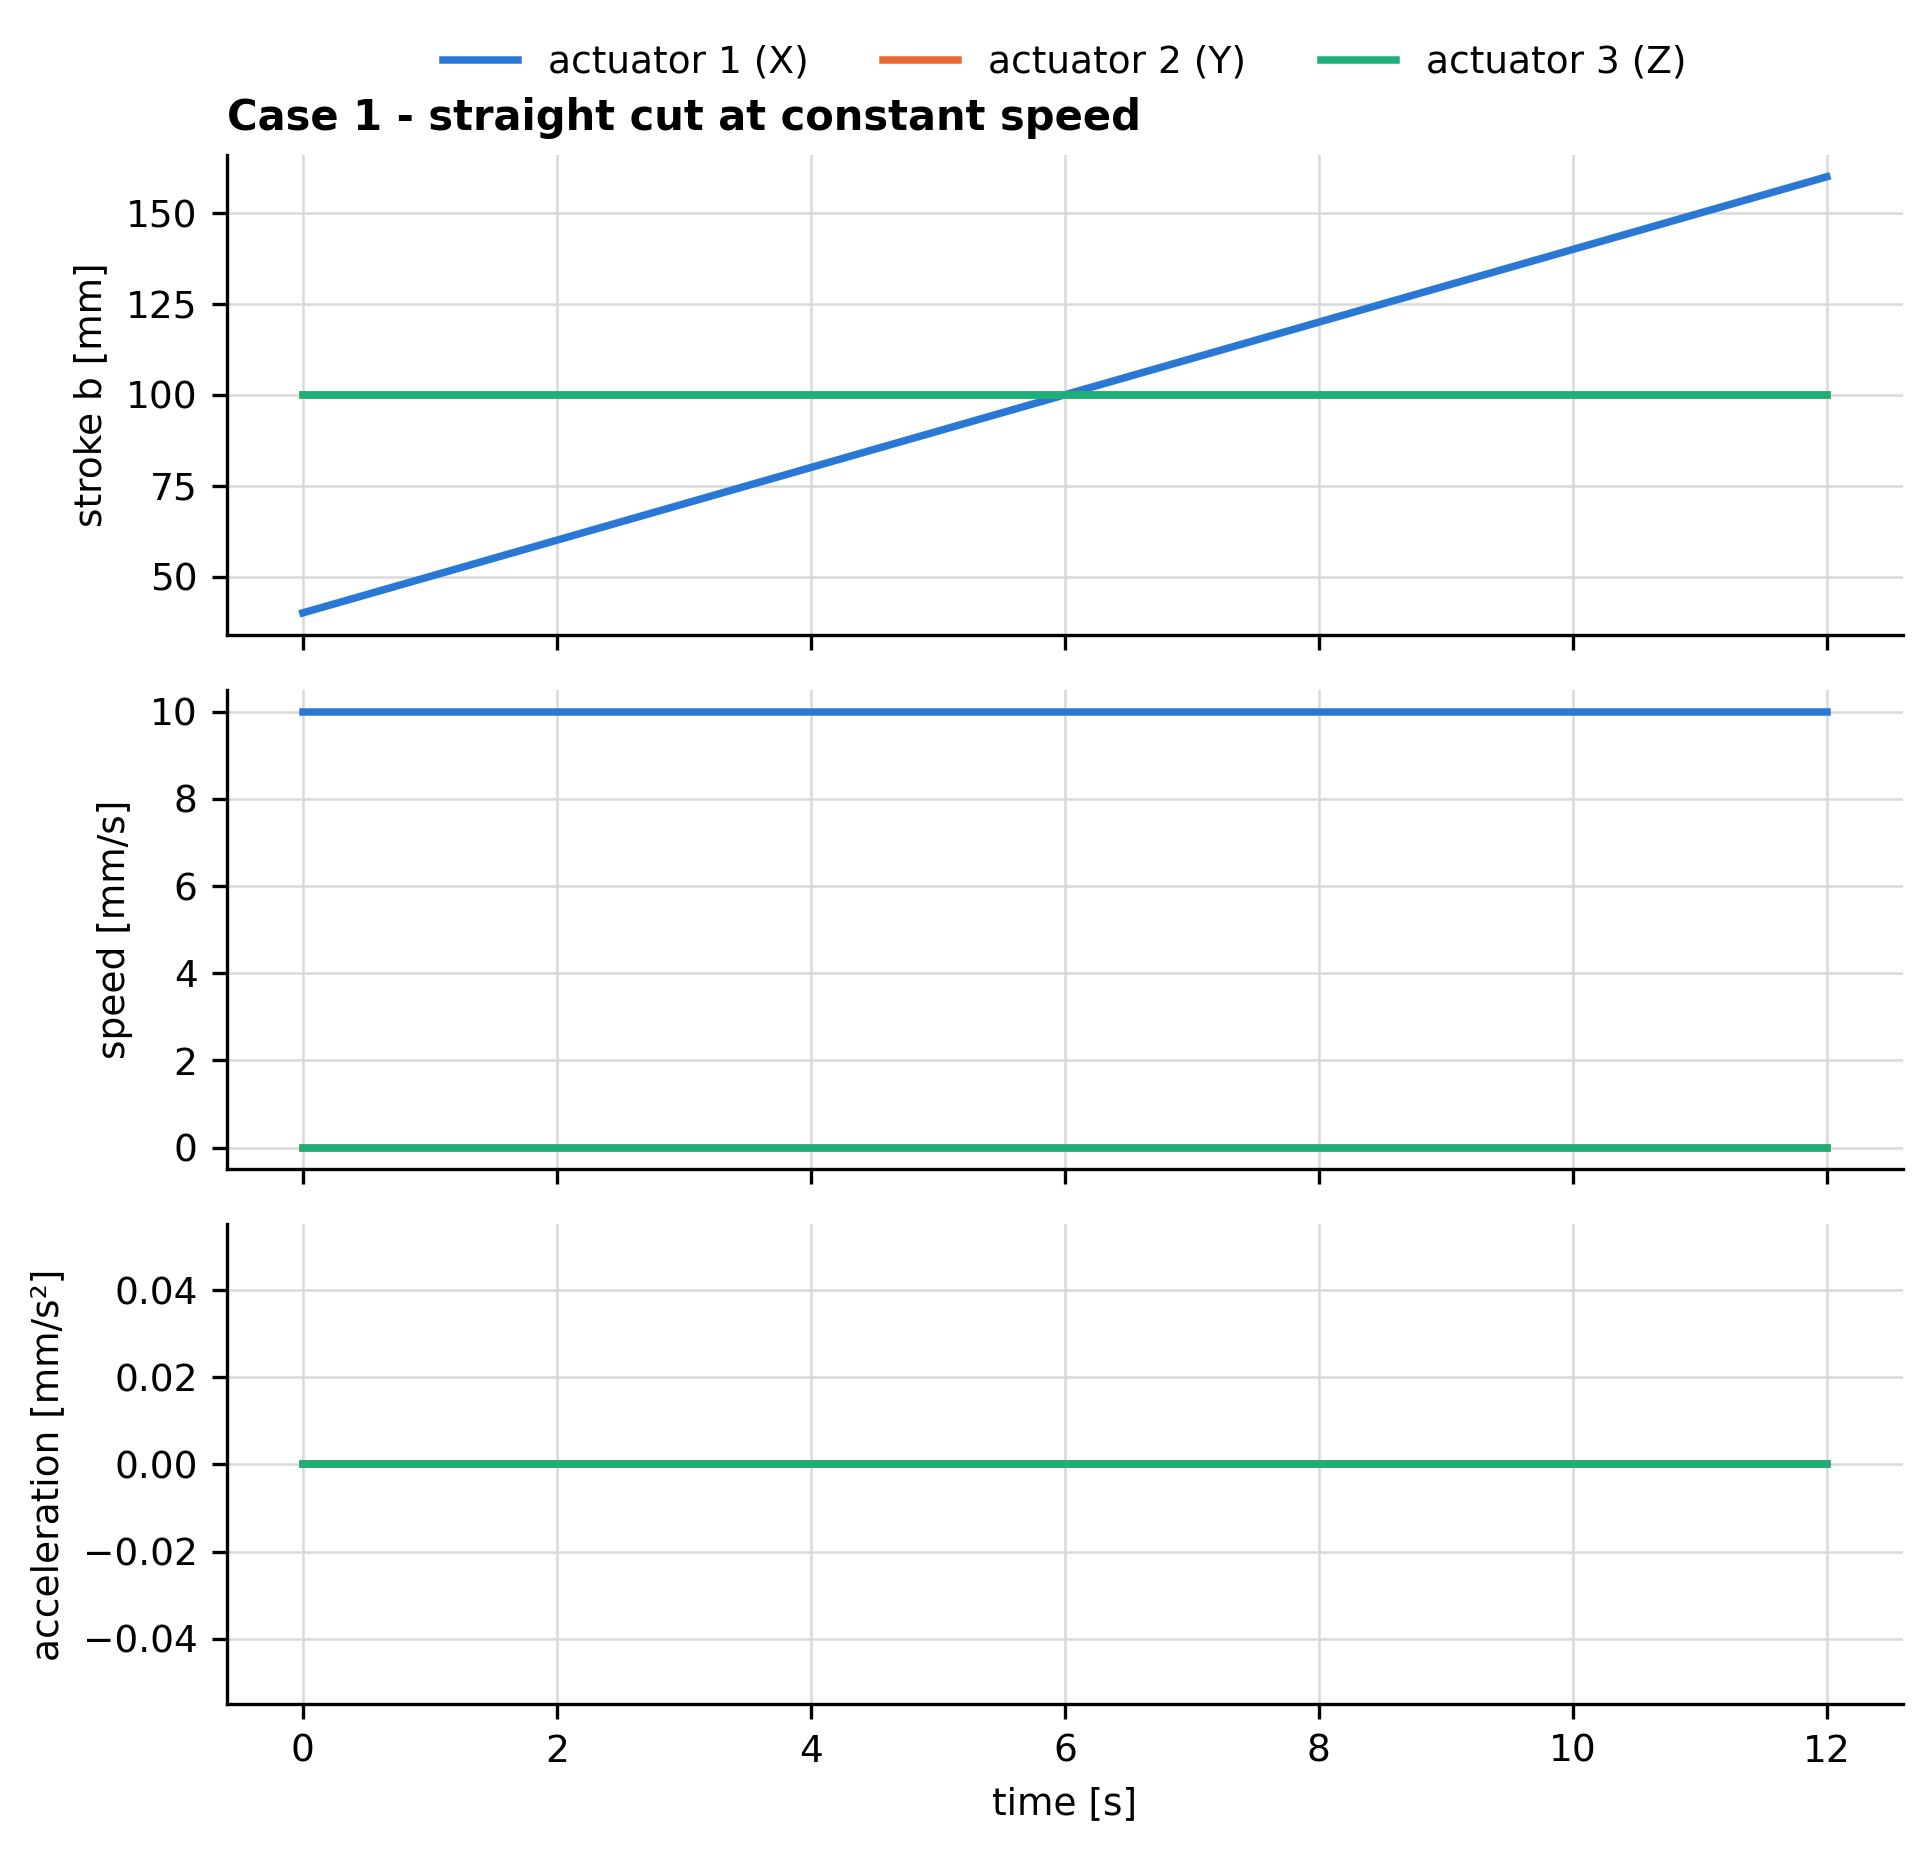
\includegraphics[width=0.92\textwidth]{figures/kinematics_case1_straight.png}
\caption{Case 1 -- straight cut: joint coordinates, speeds and accelerations.}
\end{figure}

\begin{figure}[htbp]\centering
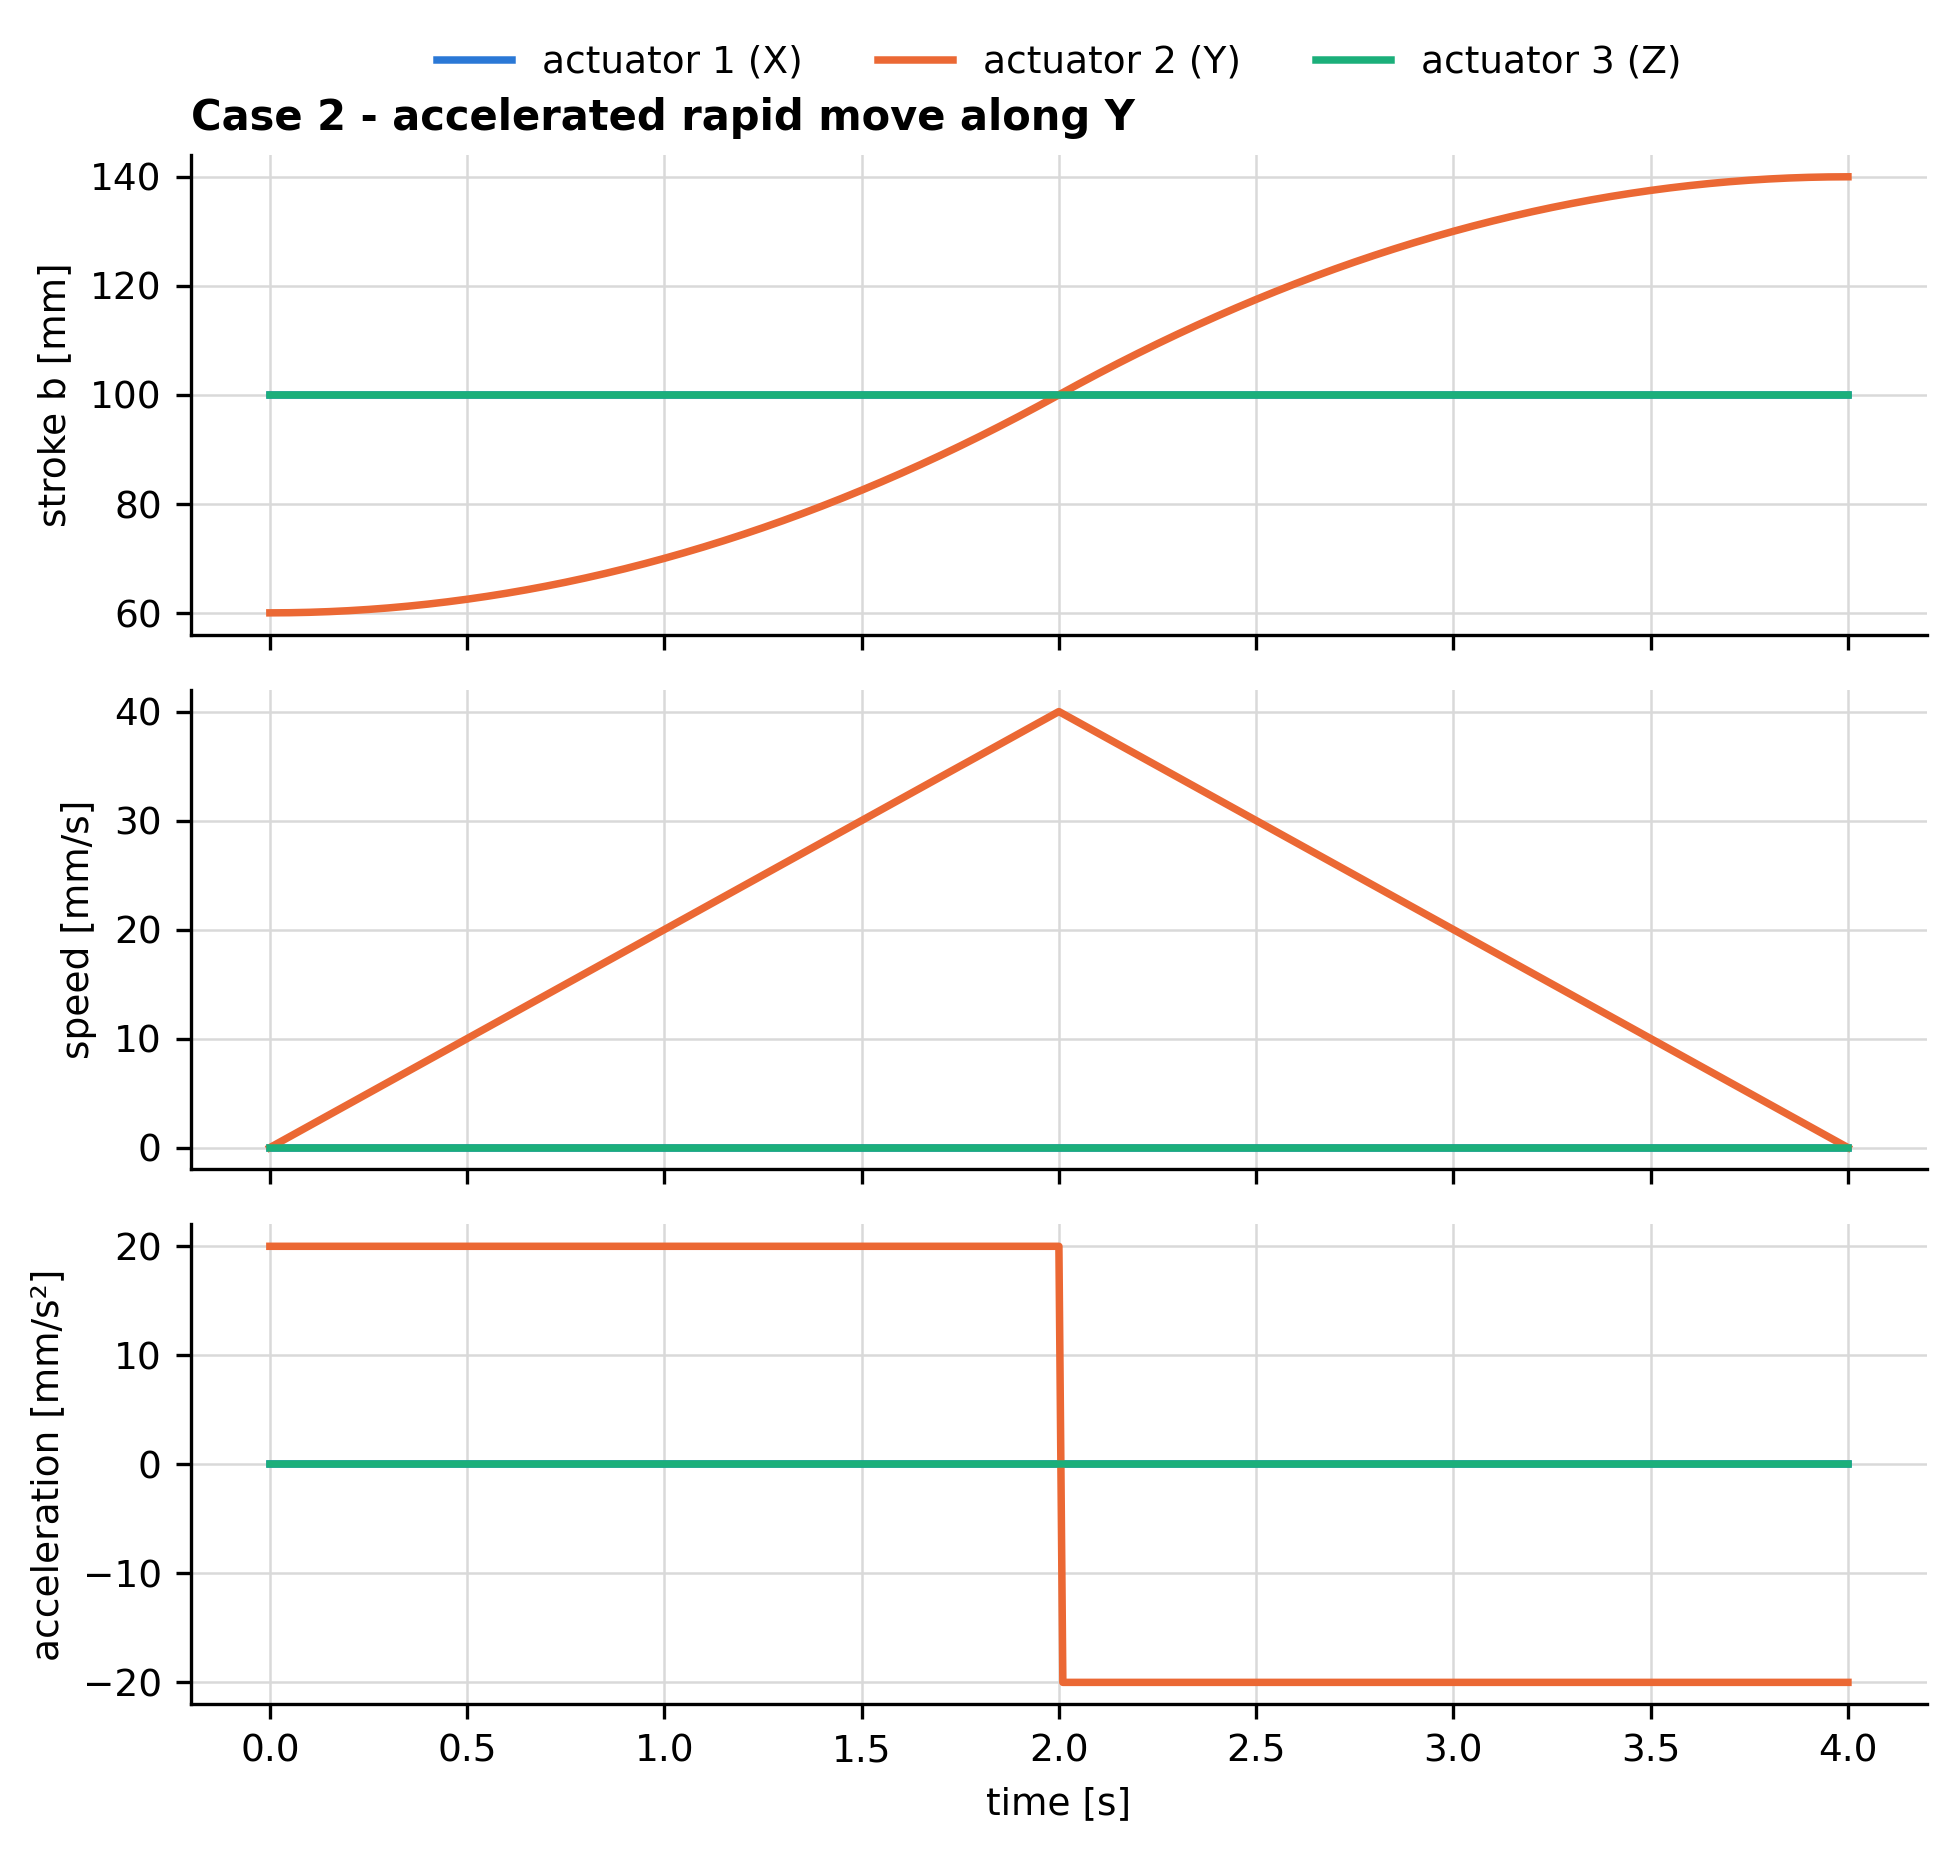
\includegraphics[width=0.92\textwidth]{figures/kinematics_case2_accelerated.png}
\caption{Case 2 -- accelerated rapid traverse along $y$.}
\end{figure}

\begin{figure}[htbp]\centering
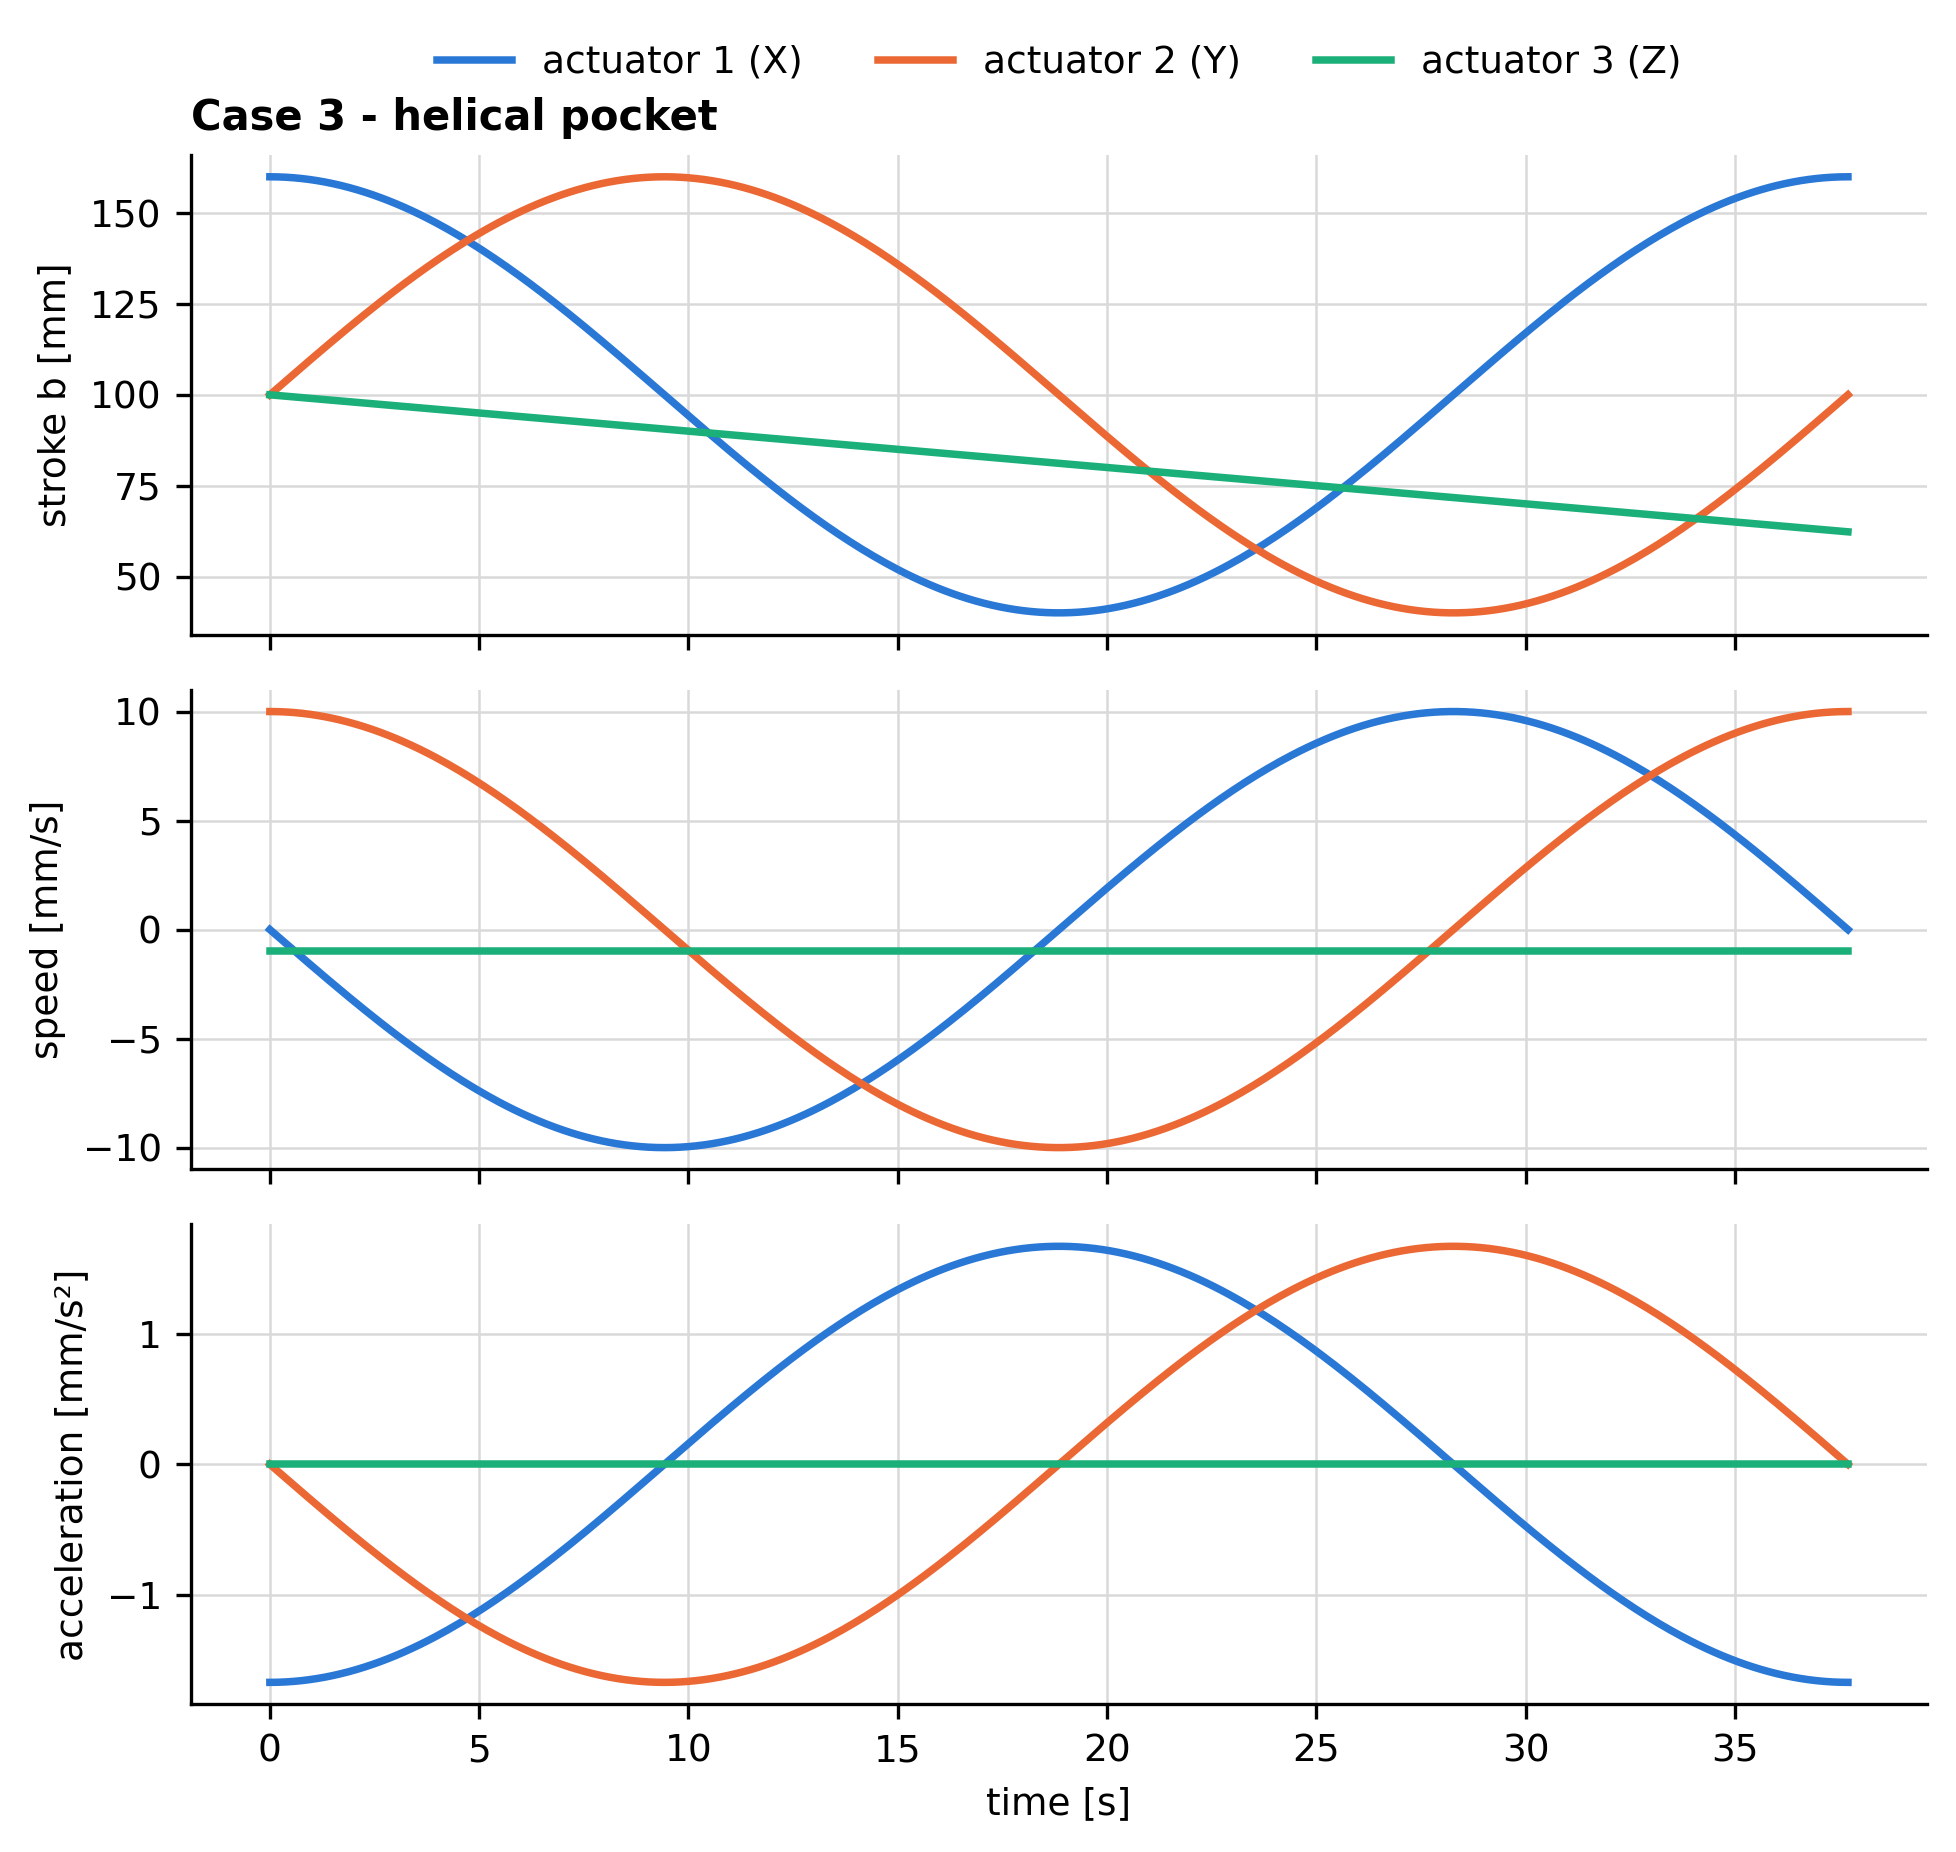
\includegraphics[width=0.92\textwidth]{figures/kinematics_case3_helical.png}
\caption{Case 3 -- helical pocketing move.}
\end{figure}

\FloatBarrier
\subsection{Workspace}

The reachable workspace was mapped by solving the inverse kinematics on a
\SI{5}{\milli\metre} grid and rejecting the poses for which any leg leaves its stroke or
any 2R chain becomes unreachable ($r>\ell_C+\ell_D$ or $r<|\ell_C-\ell_D|$). Out of
\num{68921} sampled points, the full \SI{200}{\milli\metre} cube is reachable:

\begin{center}
\begin{tabular}{@{}lc@{}}
\toprule
\textbf{Quantity} & \textbf{Value} \\
\midrule
Bounds in $x$, $y$, $z$ & $\pm\SI{100}{\milli\metre}$ each \\
Usable volume           & \SI{8.615}{\deci\metre\cubed} \\
Shape                   & Cube, no interior singularity \\
\bottomrule
\end{tabular}
\end{center}

The workspace is a perfect cube --- a direct consequence of the decoupling --- and no
singular pose was found inside it, since $\det\bm J$ keeps a constant sign over the whole
grid. This is the main practical advantage of the Tripteron over a delta or a Stewart
platform of comparable size.

\begin{figure}[htbp]\centering
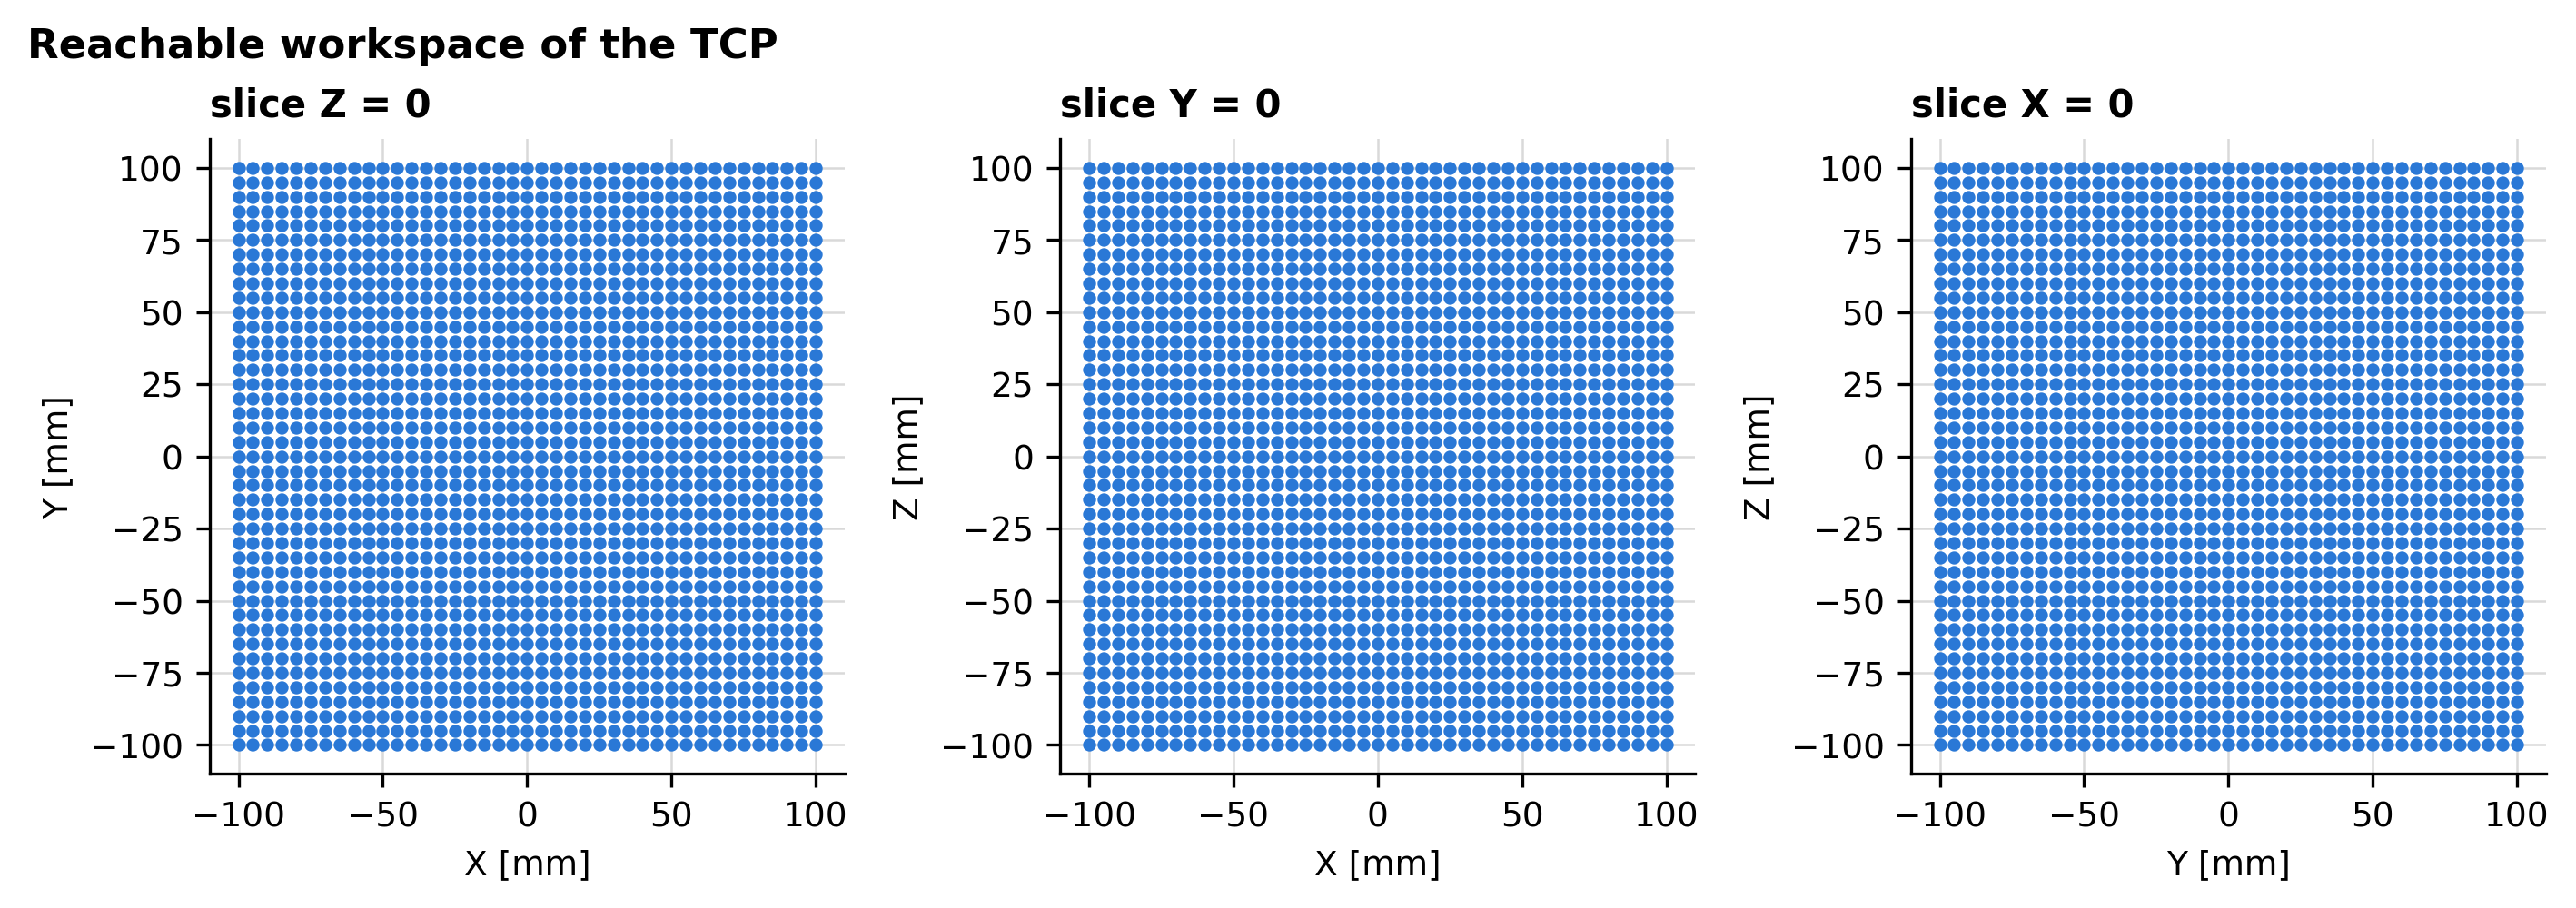
\includegraphics[width=0.78\textwidth]{figures/workspace.png}
\caption{Reachable workspace of the machine: the full \SI{200}{\milli\metre} cube.}
\end{figure}
\FloatBarrier

%==============================================================================
\sheet{Sheet 2 -- Static analysis}{J. M. Rodr\'iguez / S. Rinc\'on}
%==============================================================================
\section{Description}\label{sec:sta-desc}

With the geometry of every pose known from Sheet~1, the second calculation determines the
forces that the machine has to carry: the axial force each lead screw must produce, the
reactions at the twelve joints, and the internal bending moment of the six arms. The load
case is the cutting force at the tool tip plus the self weight of all moving bodies.

The Tripteron is an \emph{over-constrained} parallel mechanism: three closed loops share a
single platform. The rigid-body equilibrium system is therefore statically indeterminate,
and this is treated explicitly below instead of being ignored.

\section{Objective of the calculation}\label{sec:sta-obj}

\begin{enumerate}[leftmargin=*,nosep]
  \item Obtain the axial force on each actuator for the worst pose inside the workspace.
  \item Obtain the joint reactions and the maximum bending stress in the arms.
  \item Define the design axial load that Sheet~3 uses to size the lead screw.
  \item Cross-check the result with an independent energy method.
\end{enumerate}

\section{Variables of the calculation model}\label{sec:sta-var}

Each of the ten moving bodies (three carriages, six links and the platform) contributes
six equilibrium equations, and each joint contributes its unknown reaction components:
six per prismatic joint (two transverse forces, three moments and the actuator force) and
five per revolute joint (three forces and the two moments perpendicular to its axis), i.e.\
21 per leg. Assembling the whole machine gives
\begin{center}
\begin{tabular}{@{}lc@{}}
\toprule
Equilibrium equations & 60 \\
Unknown reaction components & 63 \\
Rank of the system matrix & 60 \\
Redundant (statically indeterminate) components & 3 \\
\bottomrule
\end{tabular}
\end{center}

The three redundant components are the price of the closed kinematic chains: the
platform is held by three legs where two would already fix its three translations. A
rigid-body model cannot distribute those three components; only an elastic model can.

This number is not arbitrary. The mobility count of Delivery~1 gives, for 10 moving
bodies and 12 one-degree-of-freedom joints,
$M=6\times10-12\times5=0$, while the machine evidently has three degrees of freedom.
The difference of three is precisely the number of redundant constraints introduced by
the special geometry of the Tripteron, and it reappears here as the three redundant
reaction components. The kinematic and the static models therefore agree on the degree of
over-constraint of the machine.

\section{Calculation model}\label{sec:sta-model}

\subsection{Rigid-body equilibrium}

For every body $k$ with weight $\bm W_k$ acting at its centre of mass $\bm c_k$,
\begin{equation}
\sum_j \bm R_{kj} + \bm W_k + \bm F_{\text{ext},k} = \bm 0,
\qquad
\sum_j (\bm r_{kj}-\bm c_k)\times\bm R_{kj} + \bm M_{\text{ext},k} = \bm 0
\end{equation}
where $\bm R_{kj}$ is the reaction transmitted to body $k$ at joint $j$ and
$\bm r_{kj}$ is the position of that joint. Each revolute joint transmits three force
components and the two moment components perpendicular to its axis; each prismatic joint
transmits the two force components perpendicular to its axis, the three moment components,
and the actuator force along the axis.

Collecting the unknowns in $\bm x\in\mathbb R^{63}$ gives the linear system
$\bm A\,\bm x=\bm y$ with $\bm A\in\mathbb R^{60\times63}$. Since
$\operatorname{rank}(\bm A)=60$ the system is consistent but has a three-parameter family
of solutions. The \emph{minimum-norm} solution is selected,
\begin{equation}
\bm x^{\ast}=\arg\min\lVert\bm x\rVert_2 \quad\text{subject to}\quad \bm A\bm x=\bm y,
\end{equation}
computed with a least-squares (SVD) solver. This is the physically meaningful choice for a
symmetric, equally stiff structure, and it is conservative for the arms because it does
not concentrate the redundant load in a single leg.

\subsection{Independent verification: virtual work}

The actuator forces do not depend on the redundant components, so they can be obtained
exactly from the principle of virtual work without solving the indeterminate system:
\begin{equation}
F_i = -\Bigl(\bm F_c\cdot\frac{\partial\bm P}{\partial b_i}
      + \sum_k \bm W_k\cdot\frac{\partial\bm c_k}{\partial b_i}\Bigr)
\label{eq:vw}
\end{equation}
The derivatives $\partial\bm c_k/\partial b_i$ are evaluated by central finite differences
of the position solution of Sheet~1, with a perturbation of \SI{1e-4}{\milli\metre}. This
route shares nothing with the equilibrium assembly except the geometry, so agreement
between the two is a genuine check.

\subsection{Arm stresses}

The arms are $25\times25\times\SI{2}{\milli\metre}$ square tubes:
\begin{equation}
A=\SI{184}{\milli\metre\squared},\qquad
I=\SI{16345}{\milli\metre\tothe{4}},\qquad
c=\SI{12.5}{\milli\metre},\qquad
W=\frac{I}{c}=\SI{1307.6}{\milli\metre\cubed}
\end{equation}
and the bending stress follows from the internal moment at the built-in end,
$\sigma_b=M/W$.

\section{Values of the calculation model}\label{sec:sta-val}

The cutting force is $\bm F_c=[80,\,80,\,-120]^{\mathsf T}$\,\si{\newton}: two horizontal
components from the end-mill and a vertical component pointing \emph{downwards}, i.e.\
pressing the tool into the part. Four poses were evaluated: the home pose and the three
corners of the workspace that maximise, respectively, the vertical, the diagonal and the
mixed load.

\section{Results and conclusions}\label{sec:sta-res}

\subsection{Actuator forces}

\begin{center}
\begin{tabular}{@{}lccccc@{}}
\toprule
\textbf{Pose} & $F_x$ [N] & $F_y$ [N] & $F_z$ [N] & \textbf{Worst arm} & $\sigma_b$ [MPa] \\
\midrule
Home $(0,0,0)$          & $-80.9$ & $-80.9$ & $+157.9$ & link C3 & 25.4 \\
Corner $(+90,+90,+90)$  & $-81.4$ & $-81.4$ & $+156.3$ & link C3 & 25.1 \\
Corner $(-90,-90,-90)$  & $-79.4$ & $-79.4$ & $\bm{+162.0}$ & link C3 & \textbf{26.1} \\
Corner $(+90,-90,+90)$  & $-81.4$ & $-79.4$ & $+155.0$ & link C3 & 24.9 \\
\bottomrule
\end{tabular}
\end{center}

The equilibrium residual $\lVert\bm A\bm x-\bm y\rVert$ is below
\SI{2.7e-9}{\newton} in every pose, and the actuator forces obtained from
equation~\eqref{eq:vw} agree with the equilibrium solution to better than
\SI{1e-6}{\newton}. Two completely independent methods therefore give the same answer.

\textbf{Design axial load:} $\bm{F_{\max}}=\SI{162.0}{\newton}$, at the corner
$(-90,-90,-90)$, on the vertical axis. This value is carried forward to Sheet~3.

\subsection{Interpretation}

\begin{itemize}[leftmargin=*,nosep]
  \item The horizontal actuators carry almost exactly the horizontal cutting force
        ($\approx\SI{81}{\newton}$ against \SI{80}{\newton} applied); the extra
        \SI{0.9}{\newton} is the weight of the arms projected on the horizontal axes. This
        is the expected behaviour of a decoupled machine and is a further confirmation of
        the kinematic model.
  \item The vertical actuator carries the vertical cutting force \emph{plus} the entire
        weight of the moving assembly: with the spindle off, gravity alone demands
        \SI{37.9}{\newton} on axis $z$ against \SI{0.9}{\newton} on each horizontal axis.
        The vertical screw is therefore the critical one and must never be back-driven.
  \item The variation of the actuator force across the whole workspace is only
        \SI{4.5}{\percent} ($155.0$ to \SI{162.0}{\newton}), so a single worst-case load is
        a sound basis for sizing the transmission.
  \item The maximum bending stress in the arms is \SI{26.1}{\mega\pascal} against a yield
        strength of \SI{250}{\mega\pascal} for AISI 1020, i.e.\ a safety factor of
        \textbf{9.6}. The arms are not the limiting component; they were sized by stiffness
        and by the need to accommodate the bearing bores, not by strength.
\end{itemize}

\begin{figure}[htbp]\centering
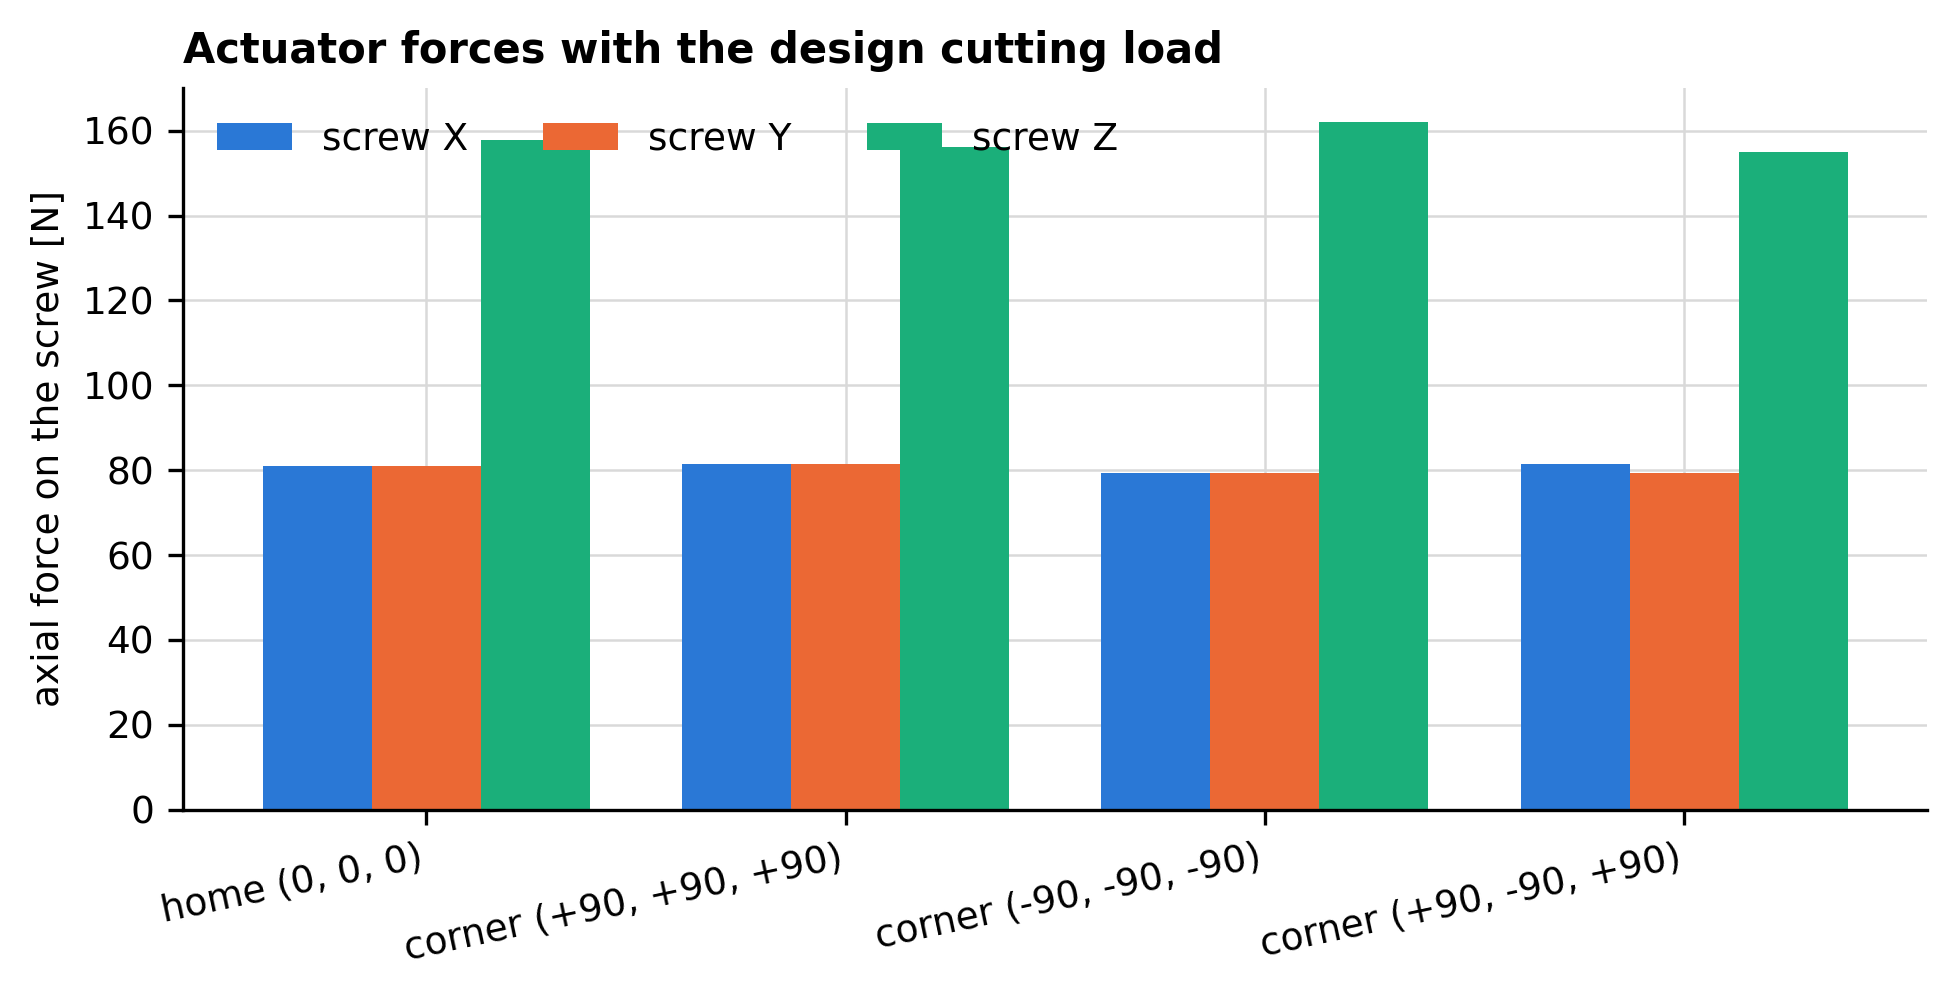
\includegraphics[width=0.92\textwidth]{figures/actuator_forces.png}
\caption{Actuator forces and worst arm bending stress for the four poses analysed.}
\end{figure}
\FloatBarrier

%==============================================================================
\sheet{Sheet 3 -- Lead-screw drive}{J. J. Garc\'ia / D. Zuluaga / G. Ria\~no}
%==============================================================================
\section{Description}\label{sec:scr-desc}

Each axis is driven by a trapezoidal lead screw turned directly by a stepper motor. The
nut is fixed to the carriage, which runs on two linear guides (the R-pair guide rails of
Delivery 2) that take all the transverse load, so the screw is loaded axially and in
torsion only. This sheet sizes that screw for the design load obtained in Sheet~2.

\section{Objective of the calculation}\label{sec:scr-obj}

\begin{enumerate}[leftmargin=*,nosep]
  \item Compute the torque required to raise and to lower the load, including collar friction.
  \item Compute the mechanical efficiency and check whether the screw is self-locking.
  \item Verify the screw body against the combined axial, torsional, thread-shear and
        bearing stresses.
  \item Verify the screw as a column in compression.
\end{enumerate}

\section{Variables of the calculation model}\label{sec:scr-var}

\begin{center}
\begin{tabular}{@{}llc@{}}
\toprule
\textbf{Symbol} & \textbf{Description} & \textbf{Value} \\
\midrule
$d$        & Nominal diameter                       & \SI{8}{\milli\metre} \\
$p$        & Thread pitch                           & \SI{2}{\milli\metre} \\
$n_s$      & Number of starts                       & 4 \\
$L$        & Lead, $L=n_s\,p$                       & \SI{8}{\milli\metre} \\
$d_m$      & Mean diameter, $d-p/2$                 & \SI{7}{\milli\metre} \\
$d_r$      & Root diameter, $d-p$                   & \SI{6}{\milli\metre} \\
$\alpha$   & Half thread angle (trapezoidal)        & \SI{15}{\degree} \\
$\lambda$  & Lead angle, $\arctan\!\bigl(L/\pi d_m\bigr)$ & \SI{19.99}{\degree} \\
$\mu$      & Thread friction coefficient (steel--bronze, greased) & 0.15 \\
$\mu_c$    & Collar friction coefficient (thrust bearing) & 0.02 \\
$d_c$      & Mean collar diameter                   & \SI{6}{\milli\metre} \\
$n_t$      & Engaged threads in the nut             & 6 \\
$\ell$     & Unsupported screw length               & \SI{500}{\milli\metre} \\
$E$        & Young's modulus, steel                 & \SI{207}{\giga\pascal} \\
$S_y$      & Yield strength                         & \SI{370}{\mega\pascal} \\
$F$        & Design axial load (Sheet~2)            & \SI{162.0}{\newton} \\
\bottomrule
\end{tabular}
\end{center}

\section{Calculation model}\label{sec:scr-model}

\subsection{Torque (Shigley, power screws)}

For a trapezoidal thread the friction coefficient is divided by $\cos\alpha$:
\begin{align}
T_R &= \frac{F\,d_m}{2}\left(\frac{L+\pi\mu d_m\sec\alpha}{\pi d_m-\mu L\sec\alpha}\right)
       + \frac{F\,\mu_c\,d_c}{2} \label{eq:TR}\\[4pt]
T_L &= \frac{F\,d_m}{2}\left(\frac{\pi\mu d_m\sec\alpha-L}{\pi d_m+\mu L\sec\alpha}\right)
       + \frac{F\,\mu_c\,d_c}{2} \label{eq:TL}
\end{align}
and the efficiency of the screw pair is
\begin{equation}
e=\frac{F\,L}{2\pi\,T_R}.
\label{eq:eff}
\end{equation}
Equation~\eqref{eq:eff} is bounded above by unity by construction. \emph{Any result above
$1$ means an arithmetic error, not a good screw.}

\subsection{Self-locking}

The screw holds the load without a brake only if the thread friction torque exceeds the
torque produced by the load, i.e.\ if the first term of~\eqref{eq:TL} is positive:
\begin{equation}
\mu \;\ge\; \frac{L\cos\alpha}{\pi d_m}.
\label{eq:selflock}
\end{equation}

\subsection{Stresses in the screw body}

With $A_r=\pi d_r^2/4$ the root area, $n_t$ engaged threads and thread thickness $p/2$ at
the root:
\begin{align}
\sigma_a &= \frac{F}{A_r}
&\tau_t &= \frac{16\,T_R}{\pi d_r^{3}} \\
\tau_{\text{thread}} &= \frac{2F}{\pi d_r\,w\,p\,n_t}
&\sigma_{\text{bearing}} &= \frac{2F}{\pi d_m\,p\,n_t}
\end{align}
where $w=0.38$ is the fraction of the pitch that the thread actually occupies at its root
on a trapezoidal profile. The body of the screw is then checked with the
distortion-energy (von Mises) criterion,
\begin{equation}
\sigma' = \sqrt{\sigma_a^2 + 3\,\tau_t^2} ,
\qquad n = \frac{S_y}{\sigma'} .
\label{eq:vm}
\end{equation}
The thread shear is \emph{not} superposed in equation~\eqref{eq:vm}: it acts on the
cylindrical surface at the root of the thread, not on the cross-section of the body, so it
is a separate check with its own margin,
$n_{\text{thread}} = 0.577\,S_y/\tau_{\text{thread}}$.

\subsection{Column buckling}

The screw is treated as a pinned--pinned column, $K=1$. With
$I=\pi d_r^4/64$, $r_g=\sqrt{I/A_r}=d_r/4$ and slenderness $\ell_e/r_g$, the transition
slenderness between the Johnson and the Euler regimes is
\begin{equation}
\left(\frac{\ell_e}{r_g}\right)_{\!1}=\sqrt{\frac{2\pi^2E}{S_y}} ,
\end{equation}
and the critical load is
\begin{equation}
P_{cr}=\frac{\pi^2EI}{(K\ell)^2}\quad\text{(Euler)},
\qquad
P_{cr}=A_r\left[S_y-\frac{1}{E}\left(\frac{S_y\,\ell_e}{2\pi r_g}\right)^{2}\right]\quad\text{(Johnson)} .
\end{equation}

\section{Values and results}\label{sec:scr-res}

\subsection{Torque and efficiency}

\begin{center}
\begin{tabular}{@{}lcc@{}}
\toprule
\textbf{Quantity} & \textbf{Design load, \SI{162.0}{\newton}} & \textbf{Delivery 1 load, \SI{151.9}{\newton}} \\
\midrule
Thread torque, raising $T_{R,\text{thread}}$ & \SI{311.9}{\newton\milli\metre} & \SI{292.5}{\newton\milli\metre} \\
Collar torque $T_c$                          & \SI{9.7}{\newton\milli\metre}   & \SI{9.1}{\newton\milli\metre} \\
\textbf{Total raising torque} $T_R$          & \textbf{\SI{321.6}{\newton\milli\metre}} & \SI{301.6}{\newton\milli\metre} \\
Total lowering torque $T_L$                  & \SI{-102.2}{\newton\milli\metre} & \SI{-95.8}{\newton\milli\metre} \\
Efficiency $e$                               & \textbf{\SI{64.1}{\percent}} & \SI{64.1}{\percent} \\
$\mu$ required for self-locking              & 0.351 & 0.351 \\
Self-locking with $\mu=0.15$?                & \textbf{No} & No \\
Fraction of motor holding torque used        & \SI{7.1}{\percent} & \SI{6.7}{\percent} \\
\bottomrule
\end{tabular}
\end{center}

\subsection{Stresses and safety factors}

\begin{center}
\begin{tabular}{@{}lcc@{}}
\toprule
\textbf{Quantity} & \textbf{Value} & \textbf{Limit / remark} \\
\midrule
Root area $A_r$                     & \SI{28.27}{\milli\metre\squared} & --- \\
Axial stress $\sigma_a$             & \SI{5.73}{\mega\pascal}  & compression \\
Torsional stress $\tau_t$           & \SI{7.58}{\mega\pascal}  & from $T_R$ \\
Thread shear $\tau_{\text{thread}}$ & \SI{3.77}{\mega\pascal}  & 6 engaged threads, $n_{\text{thread}} = 56.6$ \\
Bearing stress $\sigma_{\text{bearing}}$ & \SI{1.23}{\mega\pascal} & bronze nut, limit $\approx$ \SI{17}{\mega\pascal} \\
von Mises $\sigma'$                 & \SI{14.33}{\mega\pascal} & $S_y=\SI{370}{\mega\pascal}$ \\
\textbf{Static safety factor}       & \textbf{25.8}            & --- \\
\midrule
Second moment $I$                   & \SI{63.6}{\milli\metre\tothe{4}} & $\pi d_r^4/64$ \\
Radius of gyration $r_g$            & \SI{1.5}{\milli\metre}   & $d_r/4$ \\
Slenderness $\ell/r_g$              & 333                       & limit 105 $\Rightarrow$ Euler \\
Critical load $P_{cr}$              & \SI{519.9}{\newton}      & pinned--pinned \\
\textbf{Buckling safety factor}     & \textbf{3.21}            & --- \\
\bottomrule
\end{tabular}
\end{center}

\begin{figure}[htbp]\centering
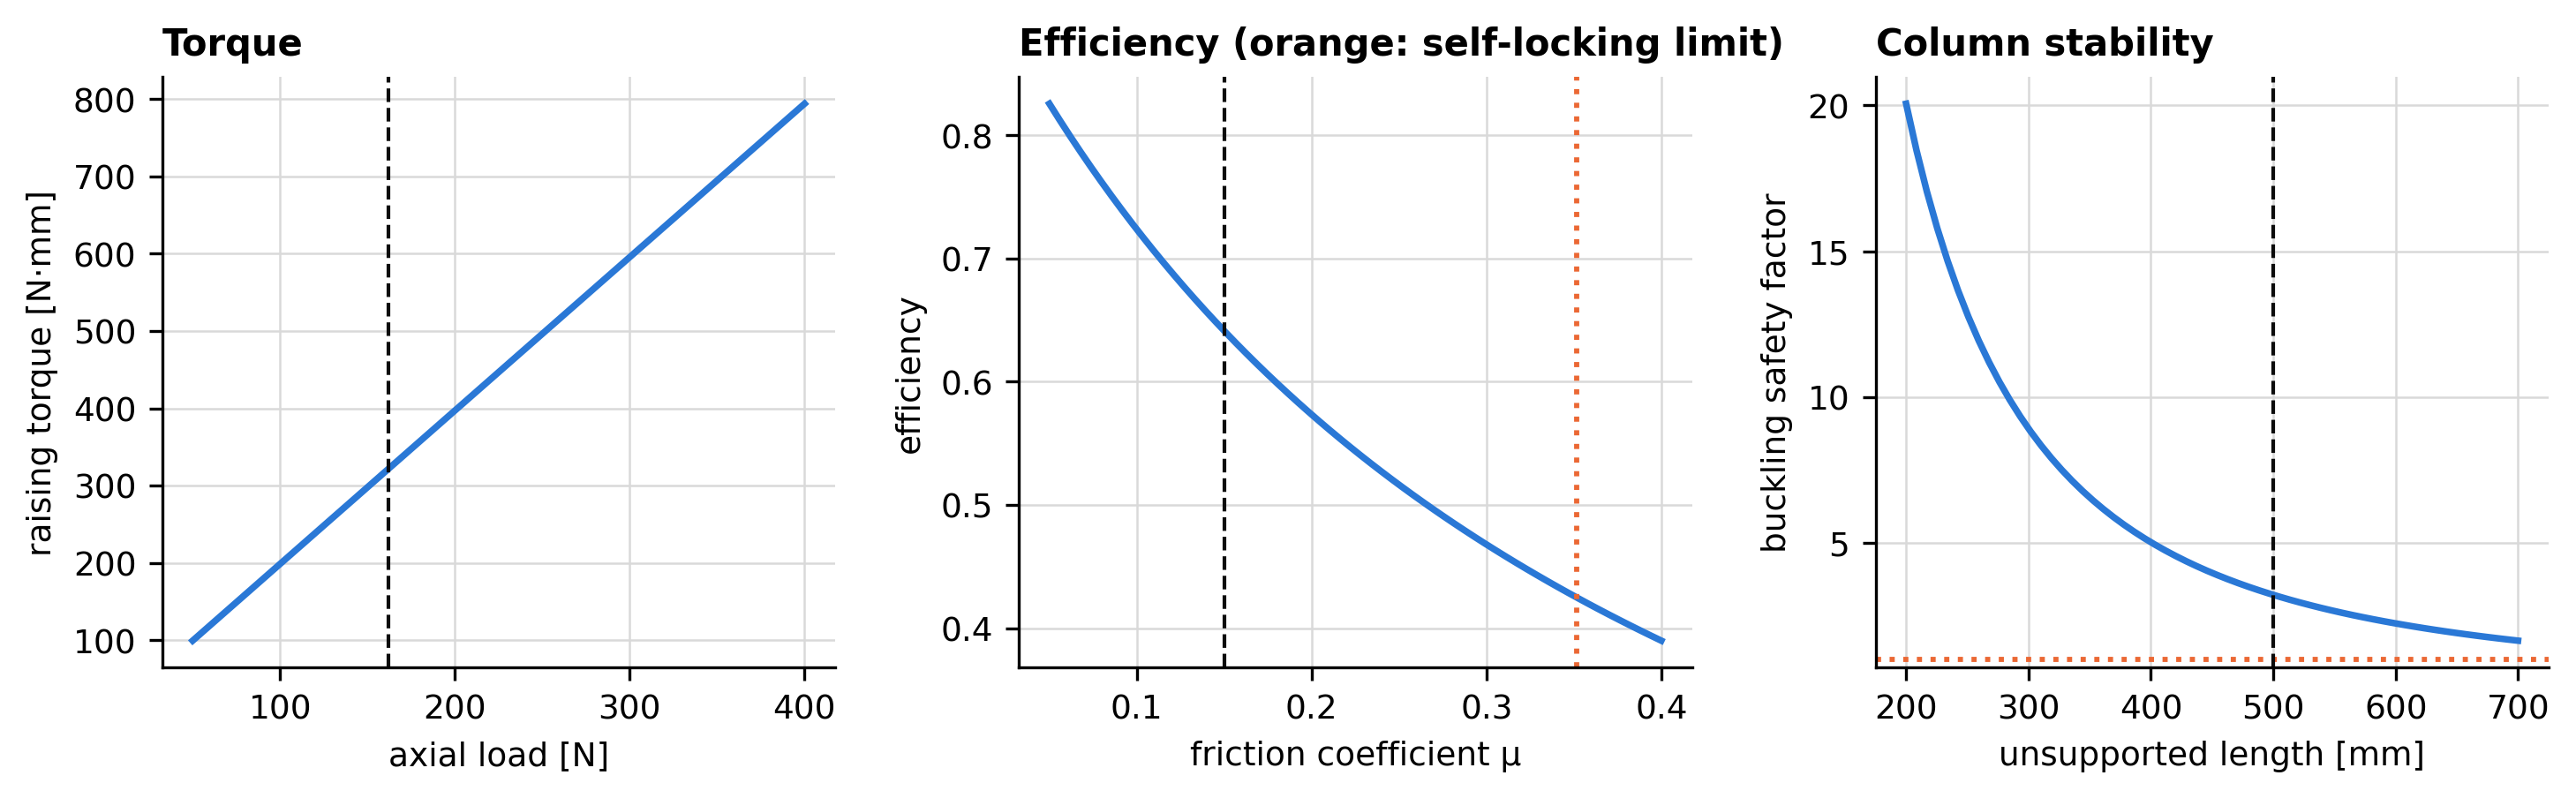
\includegraphics[width=0.92\textwidth]{figures/power_screw.png}
\caption{Lead-screw verification: torque breakdown, stress components and column check.}
\end{figure}
\FloatBarrier

\subsection{Conclusions}

\begin{enumerate}[leftmargin=*]
  \item \textbf{Strength is not the driver.} The von Mises stress of \SI{14.3}{\mega\pascal}
        gives a safety factor of 25.8. The \SI{8}{\milli\metre} screw is far stronger than
        the load requires; it was selected for availability and for the compatibility of
        its \SI{8}{\milli\metre} lead with the required feed rates.
  \item \textbf{Buckling governs the screw.} With a safety factor of 3.21 against Euler
        buckling, the column check is eight times more restrictive than the stress check.
        This is the correct behaviour for a long, slender screw and it is the criterion
        that must be re-examined if the stroke is ever increased: $P_{cr}$ falls with the
        square of the length, so a \SI{700}{\milli\metre} screw would drop to
        \SI{265}{\newton} and a safety factor of 1.6, which would no longer be acceptable.
  \item \textbf{The screw is not self-locking.} A 4-start thread has a lead angle of
        \SI{19.99}{\degree}; equation~\eqref{eq:selflock} requires $\mu\ge0.351$ while the
        greased steel--bronze pair gives $\mu=0.15$. The vertical axis \emph{will}
        back-drive under gravity if the motor is de-energised. Two consequences, both
        already covered by the selected hardware:
        \begin{itemize}[nosep]
          \item the closed-loop NEMA 34 motor must keep holding current at standstill ---
                it needs only \SI{0.32}{\newton\metre} out of \SI{4.5}{\newton\metre},
                i.e.\ \SI{7.1}{\percent} of its holding torque;
          \item an electromagnetic brake or a mechanical stop is mandatory on the $z$ axis
                for maintenance and for a power failure. This is a safety item, not an
                optional one.
        \end{itemize}
        The efficiency of \SI{64.1}{\percent} is the direct trade-off: a fast, efficient,
        non-self-locking screw.
  \item \textbf{Motor sizing is comfortable.} \SI{0.32}{\newton\metre} required against
        \SI{4.5}{\newton\metre} available leaves a factor of 14 for acceleration,
        preload, friction ageing and the inertia of the screw itself.
\end{enumerate}

%==============================================================================
\sheet{Sheet 4 -- R-pair guides and carriages}{R. Bueno / G. Ria\~no / D. Zuluaga}
%==============================================================================
\section{Description}\label{sec:gui-desc}

Each axis is guided by two parallel hardened rods on which the carriage of the R
pair slides. The nut on the lead screw takes the axial load, which Sheet~3 has already
verified; \emph{everything else} the joint has to carry --- the two transverse force
components and the three moment components --- goes through the rods and their linear
bushings. Because the arms of a Tripteron reach out from the carriage, that moment is
large, and this is the sheet that decides whether the guides can take it.

\section{Objective of the calculation}\label{sec:gui-obj}

\begin{enumerate}[leftmargin=*,nosep]
  \item Obtain the load on the most loaded linear bushing of each carriage and compare it
        with the static rating of the bushing fitted.
  \item Obtain the bending stress and the deflection of the guide rods, and compare the
        deflection with the deflection of the frame.
  \item Identify which geometric parameter of the carriage governs the result.
\end{enumerate}

\section{Variables of the calculation model}\label{sec:gui-var}

\begin{center}
\begin{tabular}{@{}llc@{}}
\toprule
\textbf{Symbol} & \textbf{Description} & \textbf{Value} \\
\midrule
$d$   & Guide rod diameter (12 H7 bore on the bearing support drawing) & \SI{12}{\milli\metre} \\
$\ell$& Clear span of the rod between end supports                     & \SI{500}{\milli\metre} \\
$b$   & Distance between the two bushings of one carriage              & \SI{60}{\milli\metre} \\
$s$   & Track width, distance between the two rods                     & \SI{115}{\milli\metre} \\
$I$   & Second moment of area of a rod, $\pi d^4/64$                   & \SI{1018}{\milli\metre\tothe{4}} \\
$W$   & Section modulus of a rod, $2I/d$                               & \SI{169.6}{\milli\metre\cubed} \\
$E$   & Young's modulus, hardened steel                                & \SI{207}{\giga\pascal} \\
$S_y$ & Yield strength of the rod                                      & \SI{350}{\mega\pascal} \\
$C_0$ & Static load rating of one linear bushing (LM12UU, catalogue)   & \SI{540}{\newton} \\
$C$   & Dynamic load rating of one linear bushing                      & \SI{390}{\newton} \\
\bottomrule
\end{tabular}
\end{center}

The rod diameter and the two spacings are read from the Delivery~2 carriage and
bearing-support drawings; the ratings are those of a standard LM12UU bushing and must be
replaced by the catalogue values of the type actually fitted before the result is used as
an acceptance criterion.

\section{Calculation model}\label{sec:gui-model}

The load case is \emph{not} assumed: it is the prismatic-joint reaction
$(\bm F_i,\bm M_i)$ that the static analysis of Sheet~2 already produced for every pose.
Splitting it along the travel axis $\bm u_i$,
\begin{equation}
\bm F_i = \underbrace{(\bm F_i\!\cdot\!\bm u_i)\,\bm u_i}_{\text{actuator, taken by the nut}}
        + \underbrace{\bm F_{t}}_{\text{transverse, taken by the bushings}},
\qquad
\bm M_i = \underbrace{(\bm M_i\!\cdot\!\bm u_i)\,\bm u_i}_{\text{roll}}
        + \underbrace{\bm M_{\perp}}_{\text{pitch and yaw}} .
\end{equation}

Each part is then reacted by a different feature of the carriage:

\begin{center}
\begin{tabular}{@{}l>{\raggedright\arraybackslash}p{5.9cm}l@{}}
\toprule
\textbf{Load} & \textbf{Reacted by} & \textbf{Bushing load} \\
\midrule
Transverse force $F_t$ & the four bushings together        & $F_t/4$ \\
Roll moment $M_{\parallel}$ & a couple between the two rods, lever arm $s$ & $M_{\parallel}/(2s)$ \\
Pitch/yaw moment $M_{\perp}$ & a couple between the two bushings of one rod, lever arm $b$ & $M_{\perp}/(2b)$ \\
\bottomrule
\end{tabular}
\end{center}

so that the worst bushing carries
\begin{equation}
F_{b} = \frac{F_t}{4} + \frac{M_{\parallel}}{2s} + \frac{M_{\perp}}{2b},
\qquad n_0 = \frac{C_0}{F_b}.
\label{eq:bushing}
\end{equation}
Superposing the three contributions on the same bushing is conservative: they reach their
maxima at slightly different poses.

The rod itself is treated as a simply supported beam of span $\ell$ with the carriage at
mid span, which is the worst position:
\begin{equation}
F_{r} = \frac{F_t}{2} + \frac{M_{\parallel}}{s},
\qquad
\delta = \frac{F_r\,\ell^{3}}{48EI},
\qquad
\sigma_b = \frac{F_r\,\ell}{4W}.
\end{equation}

\section{Results}\label{sec:gui-res}

\begin{center}
\begin{tabular}{@{}lcccc@{}}
\toprule
\textbf{Pose} & \textbf{Worst carriage} & $F_b$ [N] & $n_0=C_0/F_b$ & $\delta$ [mm] \\
\midrule
Home $(0,0,0)$         & 3 ($z$) & 188.5 & 2.86 & 0.141 \\
Corner $(+90,+90,+90)$ & 3 ($z$) & \textbf{288.6} & \textbf{1.87} & 0.146 \\
Corner $(-90,-90,-90)$ & 3 ($z$) & 143.2 & 3.77 & 0.128 \\
Corner $(+90,-90,+90)$ & 3 ($z$) & 282.8 & 1.91 & 0.154 \\
\bottomrule
\end{tabular}
\end{center}

\begin{center}
\begin{tabular}{@{}lccc@{}}
\toprule
\textbf{Worst pose, per carriage} & \textbf{Carriage 1 ($x$)} & \textbf{Carriage 2 ($y$)} & \textbf{Carriage 3 ($z$)} \\
\midrule
Transverse force $F_t$ [N]        & 23.6 & 23.6 & 0.0 \\
Pitch/yaw moment $M_{\perp}$ [N$\cdot$mm] & \num{24443} & \num{14059} & \num{34636} \\
Roll moment $M_{\parallel}$ [N$\cdot$mm]  & 0 & 0 & 0 \\
Worst bushing load $F_b$ [N]      & 209.6 & 123.1 & \textbf{288.6} \\
Rod deflection $\delta$ [mm]      & 0.146 & 0.146 & 0 \\
Rod bending stress $\sigma_b$ [MPa] & 8.7 & 8.7 & 0 \\
\bottomrule
\end{tabular}
\end{center}

\begin{center}
\begin{tabular}{@{}lcccccc@{}}
\toprule
Bushing spacing $b$ [mm] & 40 & \textbf{60 (as built)} & 80 & 100 & 120 \\
\midrule
Worst bushing load [N]   & 433.0 & \textbf{288.6} & 216.5 & 173.2 & 144.3 \\
Static safety factor     & 1.25  & \textbf{1.87}  & 2.49  & 3.12  & 3.74 \\
\bottomrule
\end{tabular}
\end{center}

\begin{figure}[htbp]\centering
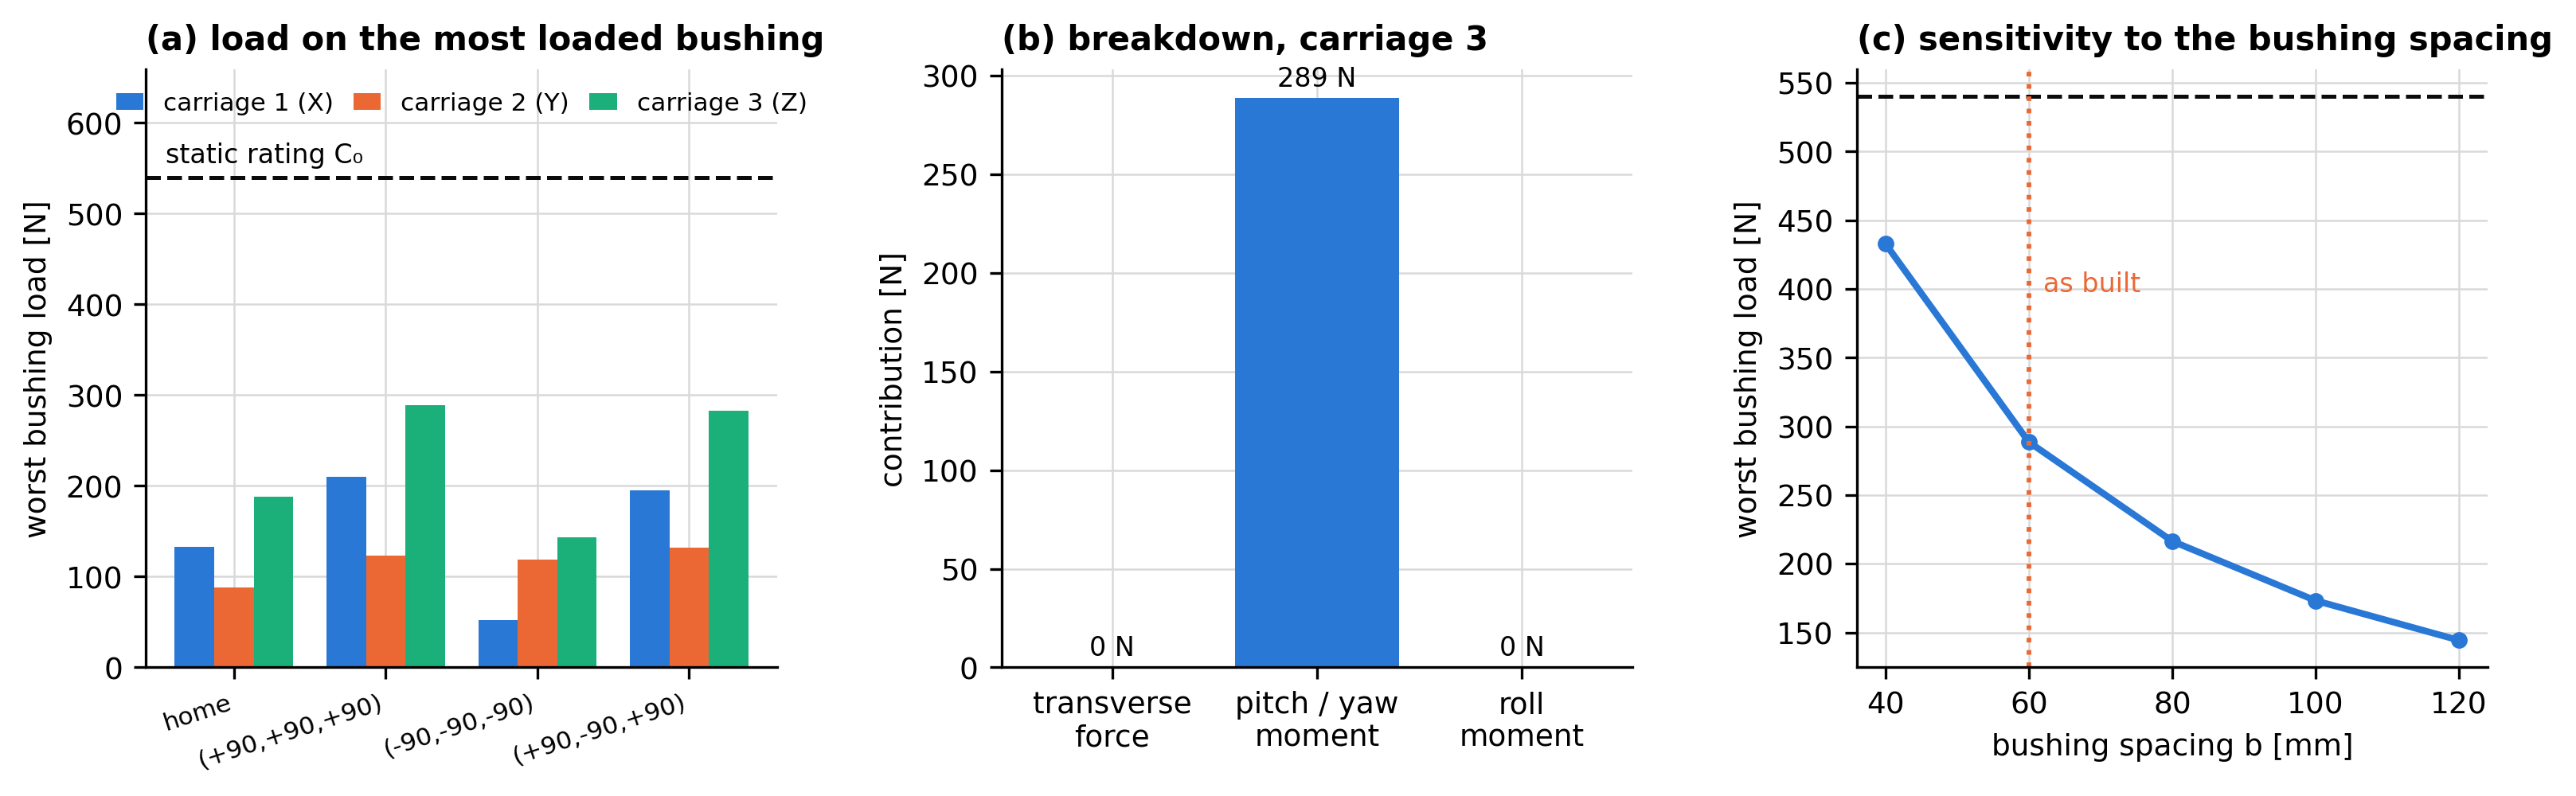
\includegraphics[width=\textwidth]{figures/guides.png}
\caption{Guide verification: load on the most loaded bushing of each carriage, where that
load comes from, and how it depends on the bushing spacing.}
\end{figure}
\FloatBarrier

\section{Conclusions}\label{sec:gui-conc}

\begin{enumerate}[leftmargin=*]
  \item \textbf{The guides carry the tightest margin in the whole machine.} With a static
        safety factor of \textbf{1.87} against the rating of an LM12UU bushing, the
        guides are more critical than the buckling of the lead screw (3.21), than the arms
        (9.6), than the screw body (25.8) and than the frame (66). Any review of this
        design should start here, not at the screw.
  \item \textbf{The load is almost entirely a moment, not a force.} On the vertical
        carriage the transverse force is zero and the whole \SI{289}{\newton} comes from
        the \SI{34.6}{\newton\metre} pitch moment that the two arms apply to the carriage.
        This is the structural signature of a Tripteron: the arms reach out from the
        carriage, so what the guide has to resist is the lever, not the cut.
  \item \textbf{The governing parameter is the bushing spacing $b$, not the rod
        diameter.} Equation~\eqref{eq:bushing} makes the moment term inversely
        proportional to $b$: moving the two bushings from \SI{60}{\milli\metre} to
        \SI{100}{\milli\metre} apart raises the safety factor from 1.87 to 3.12 at
        no cost in material. Increasing the rod diameter instead would do nothing for the
        bushing load at all. If one change is made to this machine, this is the one.
  \item \textbf{The rods are stiff enough but they dominate the machine's compliance.}
        Their bending stress is \SI{8.7}{\mega\pascal} against \SI{350}{\mega\pascal}
        (safety factor 40), so strength is irrelevant; but their worst mid-span deflection
        of \SI{0.154}{\milli\metre} is larger than the \SI{0.102}{\milli\metre} of the
        whole welded frame (Sheet~5). Guides and frame together give roughly
        \SI{0.26}{\milli\metre}, which still meets the \SI{1}{\milli\metre} accuracy
        requirement of Delivery~1, but the guides --- not the chassis --- are where the
        accuracy is lost.
\end{enumerate}

%==============================================================================
\sheet{Sheet 5 -- Chassis finite element verification}{D. Zuluaga}
%==============================================================================
\section{Description}\label{sec:fea-desc}

The three legs are mounted on a welded frame of square steel tubing that also carries the
work table. The frame is the component whose behaviour cannot be captured by a hand
calculation, because it is a three-dimensional redundant structure, so it was verified by
finite elements in SolidWorks Simulation. This sheet reports and interprets those results;
the raw nodal data exported from the solver are stored in
\texttt{04\_Calculations/data/fea\_exports/} and are post-processed by the same Python
package that produced the rest of this report, so the numbers below are not transcribed by
hand.

\section{Objective of the calculation}\label{sec:fea-obj}

\begin{enumerate}[leftmargin=*,nosep]
  \item Verify that the frame stays in the elastic range under the reactions computed in
        Sheet~2.
  \item Verify that its deflection is small compared with the machining tolerance.
  \item Verify the frame against global buckling.
\end{enumerate}

\section{Variables and model}\label{sec:fea-model}

\begin{center}
\begin{tabular}{@{}ll@{}}
\toprule
Element type      & Beam elements (welded tubular frame) \\
Material          & Alloy steel, $E=\SI{210}{\giga\pascal}$, $S_y=\SI{620}{\mega\pascal}$ \\
Boundary condition& Four feet fixed to the floor \\
Loads             & Joint reactions from Sheet~2 plus self weight \\
Studies           & Linear static + linear (eigenvalue) buckling \\
\bottomrule
\end{tabular}
\end{center}

Beam elements are appropriate here: the frame is made of slender tubes loaded mainly in
bending and axial force, welded at the nodes, and a beam idealisation reproduces that
behaviour with a fraction of the degrees of freedom of a solid mesh. Local weld stresses
are not captured by this model and are covered by the weld sizing of Delivery 2.

\section{Results}\label{sec:fea-res}

\begin{center}
\begin{tabular}{@{}lrrrr@{}}
\toprule
\textbf{Quantity} & \textbf{Samples} & \textbf{Minimum} & \textbf{Maximum} & $\lvert\cdot\rvert_{\max}$ \\
\midrule
Bending stress [MPa]        & 19 & $-9.36$   & $-0.574$  & 9.36 \\
Axial stress [MPa]          & 33 & $-0.305$  & $0.0029$  & 0.305 \\
Shear stress, dir.\ 1 [MPa] & 40 & $-0.987$  & $2.69$    & 2.69 \\
Shear stress, dir.\ 2 [MPa] & 31 & $-0.219$  & $0.627$   & 0.627 \\
Strain [--]                 & 23 & $-6.4\times10^{-6}$ & $2.9\times10^{-6}$ & $6.4\times10^{-6}$ \\
Displacement [mm]           & 22 & $0$       & $0.1016$  & 0.1016 \\
Buckling mode 1, $x$ [mm]   & 27 & $0$       & $0.0285$  & 0.0285 \\
Buckling mode 1, $y$ [mm]   & 24 & $-0.0035$ & $0.0035$  & 0.0035 \\
Buckling mode 1, $z$ [mm]   & 21 & $-0.0213$ & $0.0019$  & 0.0213 \\
\bottomrule
\end{tabular}
\end{center}

\begin{center}
\begin{tabular}{@{}lc@{}}
\toprule
\textbf{Verification} & \textbf{Result} \\
\midrule
Governing stress                  & bending, \SI{9.36}{\mega\pascal} \\
Yield strength                    & \SI{620}{\mega\pascal} \\
\textbf{Static safety factor}     & \textbf{66} \\
Maximum displacement              & \SI{0.102}{\milli\metre} \\
\textbf{Buckling load factor}     & \textbf{2238} \\
\bottomrule
\end{tabular}
\end{center}

\begin{figure}[htbp]\centering
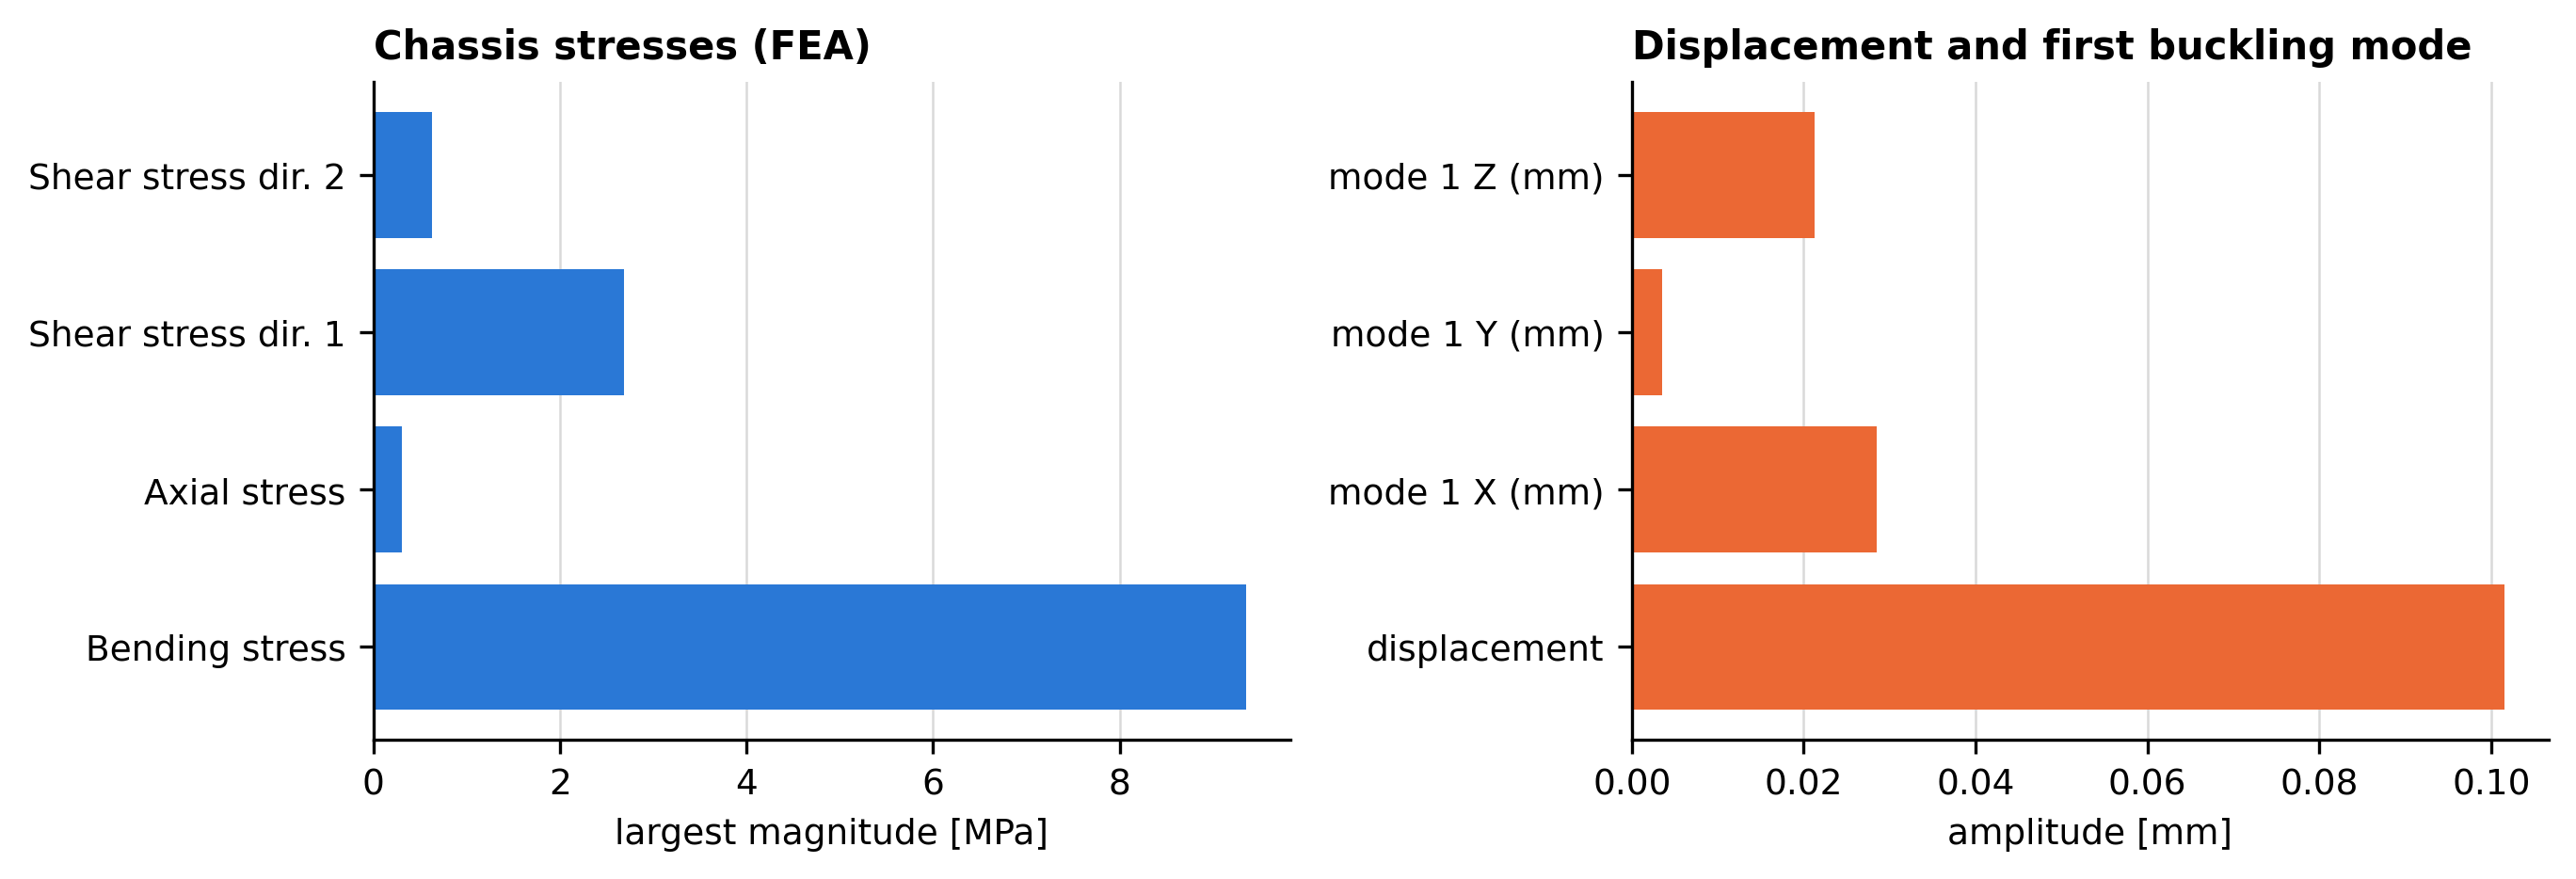
\includegraphics[width=0.92\textwidth]{figures/fea_summary.png}
\caption{Finite element results: range of each exported quantity and resulting margins.}
\end{figure}
\FloatBarrier

\section{Conclusions}\label{sec:fea-conc}

\begin{enumerate}[leftmargin=*]
  \item \textbf{The frame is massively over-strength.} A safety factor of 66 against yield
        and a buckling load factor of 2238 mean the structure is nowhere near its strength
        limit. This is not an error: the frame was sized by \emph{stiffness} and by the
        commercial tube sizes available, not by stress. In a machine tool the deflection
        under load is what shows up on the part, and it is always the binding requirement.
  \item \textbf{Stiffness is the meaningful result.} The maximum displacement of
        \SI{0.102}{\milli\metre} occurs at the top rail, furthest from the feet. Referred
        to the \SI{200}{\milli\metre} workspace this is \SI{0.05}{\percent}, and it is of
        the same order as the positioning resolution of the drives. It is acceptable for
        the intended use (light milling of aluminium and plastics) but it is the single
        number that limits the achievable accuracy of the machine, so any future increase
        of the cutting force should be checked against it first.
  \item \textbf{The dominant stress is bending}, an order of magnitude above the axial and
        shear components. The load path is therefore what one would expect: the reactions
        of the legs are applied off the neutral axis of the rails and are carried in
        bending to the feet. If the frame were ever to be lightened, the rails in bending
        are what must be preserved; the diagonal members carry little load.
  \item \textbf{Global buckling is irrelevant} for this structure at this load level. The
        first mode is a lateral sway of the uprights, and it would require 2238 times the
        service load to occur.
\end{enumerate}

%==============================================================================
\sheet{Appendix A -- Corrections}{Group 2}
%==============================================================================
\section{Corrections to the previous calculation memo}\label{sec:corrections}

The earlier version of this memo contained a number of results that cannot be correct on
physical grounds. Each of them is listed below with the reason it is wrong and the value
that replaces it. All the replacement values come from the recomputation documented in
Sheets 1--5. The page references are to the original submission,
\texttt{MemoriaCalculosGrupo2Maquinas1.pdf}, dated 25 May 2024.

\renewcommand{\arraystretch}{1.25}
\begin{longtable}{@{}p{0.5cm}>{\raggedright\arraybackslash}p{3.9cm}>{\raggedright\arraybackslash}p{4.7cm}>{\raggedright\arraybackslash}p{4.9cm}@{}}
\toprule
\textbf{\#} & \textbf{Previous result} & \textbf{Why it cannot be right} & \textbf{Corrected value} \\
\midrule
\endhead
\multicolumn{4}{@{}l}{\textbf{A. Two sheets for the same screw}}\\
\midrule
1 & The sheets \emph{Tornillo de potencia} (pp.~23--29) and \emph{Gu\'ias par R}
    (pp.~30--37) calculate the same screw and disagree on every line
  & Same formulas, different arithmetic. $T_c$: 9.114 vs.\ \SI{27.342}{\newton\milli\metre};
    $T_{\text{lower}}$: $-85.271$ vs.\ $-67.048$; $e$: 0.6202 vs.\ 1.948;
    $\sigma_a$: 3.438 vs.\ \SI{72.21}{\mega\pascal};
    $\tau_{\text{thread}}$: 0.1958 vs.\ \SI{2379.96}{\mega\pascal};
    $P_{cr}$: 93.06 vs.\ \SI{9428.8}{\newton}. At most one of each pair could be right; in
    fact both are, because the formulas themselves are wrong.
  & One screw, one sheet: Sheet~3, with $T_R=\SI{321.6}{\newton\milli\metre}$,
    $e=\SI{64.1}{\percent}$, $\sigma_a=\SI{5.73}{\mega\pascal}$,
    $\tau_{\text{thread}}=\SI{3.77}{\mega\pascal}$, $P_{cr}=\SI{519.9}{\newton}$ \\
2 & The guides themselves were never verified: the sheet titled \emph{Gu\'ias par R}
    repeats the screw calculation
  & The whole point of that sheet --- can the bushings and rods take the moment the arms
    apply to the carriage? --- is never asked.
  & New Sheet~4. The guides turn out to hold the \emph{tightest} margin of the machine,
    $n_0=1.87$ \\
\midrule
\multicolumn{4}{@{}l}{\textbf{B. Lead screw}}\\
\midrule
3 & $e_{\text{ascenso}} = 1.948$ (p.~35)
  & Efficiency above 1 would create energy. The expression was inverted, and $2$ was used
    where $2\pi$ belongs.
  & $e=FL/(2\pi T_R)=\SI{64.1}{\percent}$ \\
4 & $T = P\,\frac{d_p}{2}\,d_p\cos\theta\,f$ (pp.~25, 33)
  & Dimensionally inconsistent: it returns \si{\newton\milli\metre\squared}. It is not the
    power-screw relation, and it contains neither the lead nor the sign change between
    raising and lowering.
  & Shigley, equations~\eqref{eq:TR} and~\eqref{eq:TL} \\
5 & $T_c = \SI{27.342}{\newton\milli\metre}$ (p.~34)
  & $T_c=\mu_c F d_c/2$ with $d_c=\SI{6}{\milli\metre}$ gives a lever of
    \SI{3}{\milli\metre}, not \SI{9}{\milli\metre}. The other sheet got this one right.
  & $T_c = \SI{9.72}{\newton\milli\metre}$ at the corrected design load \\
6 & Thread shear \SI{2379.96}{\mega\pascal} (p.~36)
  & Six times the yield strength of any screw steel. The shear area was written as
    $(d_r w)^2/4A w$, which is not an area of anything.
  & $\tau=2F/(\pi d_r w p\,n_t)=\SI{3.77}{\mega\pascal}$, $n_{\text{thread}}=56.6$ \\
7 & $\sigma_a = 16 P (d_p+d_r)^2/(\pi d_r^4)$, giving \SI{3.438}{\mega\pascal} on p.~28
    and \SI{72.21}{\mega\pascal} on p.~35
  & That is a bending expression, not an axial one; an axial stress is force over area.
    Evaluated correctly the wrong formula gives \SI{72.2}{\mega\pascal}, so the
    \SI{3.438}{\mega\pascal} is also an arithmetic slip.
  & $\sigma_a=F/A_r=\SI{5.73}{\mega\pascal}$ \\
8 & $P_{cr}=2EI/\ell^2$ with $E=\SI{20000}{\mega\pascal}$, giving \SI{93.06}{\newton}
    (p.~29) and \SI{9428.8}{\newton} (p.~37)
  & The Euler load is $\pi^2EI/(K\ell)^2$, and steel has $E=\SI{207000}{\mega\pascal}$.
    The two answers differ by a factor of exactly 100, so at least one is also an
    arithmetic slip.
  & $P_{cr}=\pi^2EI/(K\ell)^2=\SI{519.9}{\newton}$, $n=3.21$ \\
9 & Slenderness $S_r=\ell/(I/A)=285.7$ with $A=4\pi d_r^2$ (p.~29)
  & Slenderness is $\ell/r_g$ with $r_g=\sqrt{I/A}$, and the area of a circle is
    $\pi d_r^2/4$, not $4\pi d_r^2$. The value was never used to choose between the Euler
    and the Johnson regime.
  & $\ell/r_g=333$ against a transition of 105 $\Rightarrow$ Euler regime \\
10 & $p=\SI{4}{\milli\metre}$ with 2 starts, yet $d_r=\SI{7}{\milli\metre}$ throughout
   & The two are incompatible: $d_r=d-p$ gives \SI{4}{\milli\metre} for $p=4$. A root
     diameter of \SI{7}{\milli\metre} corresponds to $p=\SI{2}{\milli\metre}$, which is
     the screw actually fitted.
   & Tr8$\times$8(P2), 4 starts: $p=\SI{2}{\milli\metre}$, $L=\SI{8}{\milli\metre}$,
     $d_m=\SI{7}{\milli\metre}$, $d_r=\SI{6}{\milli\metre}$ \\
11 & Self-locking claimed for the vertical axis
   & Consequence of \#10. A 4-start screw with $\mu=0.15$ cannot be self-locking.
   & Not self-locking; a brake or permanent holding current is required on $z$ \\
\midrule
\multicolumn{4}{@{}l}{\textbf{C. Statics}}\\
\midrule
12 & ``27 equations and 27 unknowns'', ``8 bars with 9 binary revolute pairs'' (p.~3)
   & The machine has 10 moving bodies and 12 joints. The three prismatic joints were left
     out of the model altogether.
   & 60 equations, 63 unknowns, rank 60, 3 redundant reactions \\
13 & The actuator forces never appear in the results (p.~7)
   & They are the reason a static analysis is done at all: without them the screw and the
     motor cannot be sized. Leaving the prismatic joints out of the model removed them.
   & $F_x=F_y=\SI{-80.9}{\newton}$, $F_z=\SI{+157.9}{\newton}$ at home; design load
     \SI{162.0}{\newton} \\
14 & Reactions of 0 to \SI{10}{\newton}, most of them exactly zero (p.~7)
   & A \SI{120}{\newton} cutting force cannot produce \SI{5.77}{\newton} of reaction. An
     all-zero solution is the trivial solution of a system assembled without its load
     vector.
   & Residual below \SI{3e-9}{\newton}, cross-checked by virtual work \\
15 & Cutting force applied upwards
   & An end mill pushes the work downwards against the table; applied upwards it cancels
     part of the weight of the moving assembly and under-predicts the load on the vertical
     screw.
   & $\bm F_c=[80,80,-120]^{\mathsf T}$\,\si{\newton} $\Rightarrow$ design load
     \SI{162.0}{\newton} instead of \SI{85}{\newton} \\
\midrule
\multicolumn{4}{@{}l}{\textbf{D. Kinematics and presentation}}\\
\midrule
16 & No verification of the kinematic solution
   & A position solution with no residual and no independent check cannot be audited.
   & Newton--Raphson residual below \SI{8e-11}{\milli\metre}, agreement with the
     closed-form inverse kinematics to $10^{-13}$\,mm, velocities and accelerations
     checked against finite differences \\
17 & The chassis sheet (pp.~38--60) carries no date and no reviewer
   & An unsigned, undated calculation sheet cannot be released.
   & Every sheet of this edition carries project, calculation, analyst, reviewer, date and
     page \\
\bottomrule
\end{longtable}
\renewcommand{\arraystretch}{1}

\subsection{Effect of the corrections on the design}

None of the corrections invalidates the machine. The two that matter in practice are:

\begin{itemize}[leftmargin=*,nosep]
  \item \textbf{Correction 8} raises the design axial load from \SI{85}{\newton} to
        \SI{162.0}{\newton}. The screw still passes every check, but the buckling safety
        factor drops from about 6 to 3.21, which is why the column check --- and not the
        stress check --- is now the governing criterion for the transmission.
  \item \textbf{Correction 11} changes an operating requirement: the vertical axis is not
        self-locking and needs a brake or a permanently energised motor. This is a safety
        item that the previous memo did not identify.
  \item \textbf{Correction 2} changes where the attention should go. Because the sheet
        that was supposed to verify the guides verified the screw instead, nobody ever
        computed the load on the bushings. It turns out to be the tightest margin in the
        machine ($n_0=1.87$), and it is fixed by moving two bushings further apart --- the
        cheapest change available anywhere in this design.
\end{itemize}

%==============================================================================
\sheet{Appendix B -- Calculation software}{Group 2}
%==============================================================================
\section{Reproducing the results}\label{sec:software}

Every figure and every number in this report is generated by the Python package stored
in the folder \texttt{04\_Calculations}. A single command regenerates all of them:

\begin{center}\ttfamily
python run\_all.py
\end{center}

The script creates its own virtual environment on first use, installs the dependencies and
writes the results to \texttt{results/} (CSV and JSON) and \texttt{figures/} (PNG).

\begin{center}
\begin{tabular}{@{}l>{\raggedright\arraybackslash}p{9.6cm}@{}}
\toprule
\textbf{Module} & \textbf{Contents} \\
\midrule
\texttt{parameters.py}     & All machine data in one place: geometry, masses, materials, loads. \\
\texttt{kinematics.py}     & Constraints, Jacobian, $\dot{\bm J}$, Newton--Raphson solver, closed-form inverse kinematics, trajectory generation, workspace mapping. \\
\texttt{statics.py}        & Assembly of the 60$\times$63 equilibrium system, minimum-norm solution, virtual-work actuator forces, arm section properties and bending stresses. \\
\texttt{power\_screw.py}   & Screw geometry, raising/lowering torque, efficiency, self-locking, stresses, Euler/Johnson column check. \\
\texttt{guides.py}         & Splits the prismatic-joint reaction into transverse force, roll and pitch/yaw moment; bushing loads, rod stress and deflection, sensitivity to the bushing spacing. \\
\texttt{fea\_postprocess.py}& Reads the nodal data exported from SolidWorks Simulation and computes the ranges and safety factors of Sheet~4. \\
\texttt{run\_all.py}       & Runs the four studies and writes results and figures. \\
\bottomrule
\end{tabular}
\end{center}

\subsection{Verification strategy}

Each physical result is produced by two independent routes, and the report states the
discrepancy between them:

\begin{center}\small
\begin{tabular}{@{}>{\raggedright\arraybackslash}p{3.4cm}>{\raggedright\arraybackslash}p{6.1cm}>{\raggedright\arraybackslash}p{6.6cm}@{}}
\toprule
\textbf{Result} & \textbf{Method 1} & \textbf{Method 2} \\
\midrule
Position   & Newton--Raphson on $\bm\Phi(\bm q,t)=\bm 0$ & Closed-form 2R inverse kinematics \\
Velocity, acceleration & Analytical $\bm J$, $\dot{\bm J}$ & Finite differences of the position solution \\
Actuator forces & 60$\times$63 rigid-body equilibrium & Principle of virtual work \\
Screw & Shigley closed-form expressions & Dimensional and physical bounds ($e\le1$, $\sigma<S_y$) \\
Guides & Prismatic-joint reactions of Sheet~2 & Free-body couple check on the carriage \\
Chassis & Finite elements & Order-of-magnitude hand check of the rails in bending \\
\bottomrule
\end{tabular}
\end{center}

\vspace{8pt}
\begin{center}
\rule{0.6\textwidth}{0.4pt}\\[6pt]
\textit{End of report}
\end{center}

\end{document}
